\documentclass[uplatex]{jsarticle}

\renewcommand{\labelenumii}{\theenumii}
\renewcommand{\theenumii}{\theenumi.\arabic{enumii}.}

% Font
\usepackage[uplatex]{otf}
% \usepackage{times}

% Graphics
\usepackage[dvipdfmx,hiresbb]{graphicx}
\usepackage{array, booktabs}
\usepackage{subcaption}

% Algorithm
\usepackage{algorithm}
\usepackage{algorithmic}
\captionsetup[algorithm]{labelformat=empty}

% index
\usepackage{makeidx}
\makeindex

% Hypertext
\usepackage[dvipdfmx]{hyperref}

% Utility
\usepackage{comment}

% Style
%\usepackage{ijcai15}

\title{マルチコアマシンにおける\\
並列A*探索の探索オーバーヘッドの定性的な解析と\\
アルゴリズムの再評価}
\author{陣内 佑 \\
東京大学教養学部学際科学科\\
\\
指導教員 福永 Alex}

\begin{document}

\maketitle
\thispagestyle{empty}

% HDA*もPBNFも既存研究である。KishimotoらはHDA*のin depth analysisをしているし、HDA* vs PBNFの性能比較実験もBurnsらによってなされている。第一印象では、この実験はただの焼き増しである。早急にこの誤解を解く必要がある。
\begin{abstract}
% Why study A*?
グラフ探索問題のうち最も重要なものの一つとして、辺にコストのついた有向グラフ、初期状態、ゴール状態を入力とし、初期状態からゴール状態までの経路のうちコストが最小である経路を出力する問題がある。この問題を解く為の代表的なアルゴリズムのフレームワークとしてA*探索がある。このA*探索を並列化する手法は数多く提案されている。

% Why study HDA*?
HDA*は特に分散メモリ環境において効率的な並列A*探索である。
HDA*は各スレッドに対してオープンリスト・クローズドリストをローカルに置き、スレッド間で非同期的に仕事を分配する。HDA*は探索済のノードの全てをクローズドリストに保存する為、TDSなどの探索済ノードの一部しか保存しないアプローチと比較して余剰な展開ノードが少ない。しかしHDA*はPBNFと比較して余剰な展開ノードが生じるという先行研究が存在する。PBNFは共有メモリ環境においてstate-of-the-artとされる手法である。PBNFがHDA*よりも優れる理由としては余剰な展開ノードの数が小さいことが指摘されている。しかしながら、先行研究によるHDA*とPBNFの性能比較実験は複数問題点がある。

% What am I going to do?
本研究はまず、HDA*の余剰な展開ノードを定性的に分析し、その原因を3つに分類する。また、問題サイズが十分に大きい場合、それらのオーバーヘッドが無視出来る大きさであることを理論的・実験的に示す。
次に、先行研究におけるHDA*とPBNFの性能比較実験の問題点を指摘し、その上でより詳細な性能比較実験を行う。その実験結果として、 (1) 両アルゴリズムで展開ノード数は大きく変わらないこと、 (2) 逐次実行で10秒程度以上の問題ではHDA*の方がパフォーマンスに優れることを示す。
\end{abstract}

\newpage
\tableofcontents
\thispagestyle{empty}
\newpage

\section{序論}
\setcounter{page}{1}

\subsection{研究の背景}
% Why should we study this?
グラフは情報科学に通底する問題ドメインであり、グラフを解き明かす探索アルゴリズムは分野の基本骨子をなしている。人工知能の分野においても探索は基盤となるアルゴリズムの一つであり、高速で効率的な探索アルゴリズムを研究することは人工知能於いては情報科学全体に意義のある研究である。さて、近年単一プロセッサの高速化は電力の限界を迎え、並列化による高速化へとパラダイムが移った。ハードウェアは今後も各CPUの計算速度の発展よりも並列化による高速化が進むだろうと予測されている。
故に今後ハードウェアの高速化の恩恵を引き出す為にはこの並列システムを利用したアルゴリズムを開発する必要がある。然るに探索アルゴリズムも単一プロセッサによる探索だけではなく、マルチコア・分散システムにおいてもそれぞれ効率的なアルゴリズムを研究しなければならない。


\subsection{関連研究}

グラフを探索するアルゴリズムのうち最も重要なものの一つとしてA*(エースター)アルゴリズムがある\cite{Hart1968}。このA*アルゴリズムを並列化する手法は数多く提案されている。

% 簡単な説明バージョン

% Parallel A*
Kumarらはオープンリスト, クローズドリストをスレッド間で共有して並列に探索を行うParallel A*を提案した。Parallel A*は非常にシンプルな手法であるが、データ構造を共有するために同期オーバーヘッドが非常に大きいという問題がある。\ref{sec:analysis2}章で見るように、このシンプルな手法は逐次A*よりも遅くなってしまう。

% HDA*
同期オーバーヘッドを解決する手法として、KishimotoらはHash Distributed A* (HDA*)を提案した\cite{Kishimoto2013}。HDA*では、各スレッドがそれぞれローカルにオープンリストとクローズドリストを持つ。グラフのノードはHash関数によって均等かつ無作為に分割し各スレッドに割り当てられる。各スレッドは自分に割り当てられたノードのみを展開し、他スレッドに割り当てられたノードを生成した場合はそのスレッドにノードを非同期的に送信する。HDA*は各スレッドがローカルのデータ構造にしかアクセスしない為、同期オーバーヘッドが殆どない。その為、HDA*は特に分散メモリ環境で効率的であるとされている。

% PBNF
Parallel Best-NBlock-First (PBNF, SafePBNF)は余剰な展開ノード数を小さくすることを目的として設計された共有メモリ環境における並列探索アルゴリズムである\cite{Burns2010}。理想的には、全てのスレッドは最も有望なノードを探索する。PBNFはこれを実現するために、状態空間を複数のnblockに分割し、それぞれのスレッドが最も有望なノードを持つnblockを占有して探索する。PBNFは分散メモリ環境では有効ではないが、現在共有メモリ環境で最もパフォーマンスの良いstate-of-the-artの手法であるとされている。

% Why this research is important?
Burnsらは共有メモリ環境でPBNFとHDA*を含めた9つの並列アルゴリズムの性能比較を行い、その中でPBNFとHDA*を最も有望な(高速な)アルゴリズムとした。その上でPBNFはHDA*よりパフォーマンスに優れると結論をした。その理由として、PBNFがHDA*よりも展開ノード数が小さいという結果があったことを指摘した。しかしながら、Burnsらの比較実験には二つ問題点がある。一つに、Burnsらの実験におけるHDA*のHash関数の実装は最適なものではなかった。もう一つは、ベンチマーク問題のサイズが小さいということが挙げられる。並列アルゴリズムは初期化に時間がかかる為、ある程度問題サイズが大きいものでないと実質的な高速化効率を正確に測ることが出来ない。よって、適切な実験設定の元で両アルゴリズムを再評価することは有意義である。一方、HDA*の展開ノード数の増加の原因はまだ研究されていない。HDA*だけでなく、並列探索アルゴリズムの展開ノード数の増加の原因を定性的に分析する事例は非常に少ない。

\begin{comment}
% Parallel A*の説明
Kumarらはオープンリスト, クローズドリストをスレッド間で共有して並列に探索を行うParallel A*を提案し、性能評価を行った\cite{Kumar1988parallel}。この手法はオープンリスト, クローズドリストのデータ構造を保つ為に相互排他ロックを必要とする。ノードが展開される度にオープンリストに、生成される度にクローズドリストにロックを獲得してアクセスする必要がある。その為Parallel A*は同期オーバーヘッドが非常に大きいという問題がある。\ref{sec:analysis2}章で見るように、このシンプルな手法は逐次A*よりも遅くなってしまう。
\newline

% HDA*の説明
同期オーバーヘッドを解決する手法としてKishimotoらはHash Distributed A* (HDA*)を提案した\cite{Kishimoto2013}。HDA*は各スレッドにローカルにオープンリストとクローズドリストを持つ。グラフのノードはHash関数によって均等かつ無作為に分割し各スレッドに割り当てられる。各スレッドは自分に割り当てられたノードのみを展開し、他スレッドに割り当てられたノードを生成した場合はそのスレッドにノードを非同期的に送信する。各スレッドのオープンリスト、クローズドリストは他のスレッドからアクセスされないので、相互排他ロックを必要としない。その為HDA*は同期オーバーヘッドが殆どない。HDA*は同期オーバーヘッドが殆どなく、スレッド間でノードの送信以外に大きな情報の通信を必要としないので、特に分散メモリ環境で有効な手法である。また、アルゴリズムの論理が非常にシンプルであるという利点もある。HDA*は逐次A*と比較してHash関数による分配が必要なだけであり、各スレッドの処理は逐次A*と殆ど同様である。並列アルゴリズムはデバッグが難しい為、シンプルであるということは非常に価値がある。HDA*の問題点としても、展開ノード数が大きくなることが指摘されている。HDA*において展開ノード数が増加する原因はまだ調べられていない。また、Kishimotoらの性能評価は殆ど分散メモリ環境におけるものであり、共有メモリ環境における実験は殆ど行われていない。また、それらも共有メモリ環境に最適化された実装を用いたものではない。その為、HDA*のマルチコアマシンにおける性能評価は不十分であると言える。
\newline

% PBNF IMPV: 複雑さをもっとうまく説明出来ないか。
Burnsらは共有メモリ環境における並列化手法としてParallel Best-NBlock-First (PBNF)を提案した\cite{Burns2010}。PBNFは状態空間を複数のnblockに分割する。それぞれのnblockはオープンリストとクローズドリストを持つ。それぞれのスレッドは最も有望なノードを持つnblockを占有し、探索を行う。自分の占有しているnblockよりも有望なノードを持つnblockが空いていれば、今探索していたnblockを解放し、新しいnblockを占有して探索を始める。あまりに頻繁なnblockの切り替えが生じるのを防ぐために最小展開ノード数が設定される。これはチューニングの必要なパラメータである。nblockはスレッドに占有されるので、オープンリスト・クローズドリストに相互排他ロックをかける必要がない。必要なロックは空いているnblockを保存するheapのみである。その為PBNFは同期オーバーヘッドが小さい。PBNFは分散メモリ環境では有効ではないが、現在共有メモリ環境で最もパフォーマンスの良いstate-of-the-artの手法であるとされている。PBNFの問題点として、その複雑さが挙げられる。すなわち、PBNFのパフォーマンスを引き出す為には空間をnblockに分割する方法・粒度と最小展開ノード数をドメインに対して最適化をする必要がある。
\newline


% HDA* vs PBNF比較実験の問題点: 何故再実験する価値があるのか
BurnsらはマルチコアマシンでHDA*を含めた様々な並列アルゴリズムの性能比較を行い、その中でPBNFとHDA*を有望な(高速な)アルゴリズムとした。その上でPBNFはHDA*よりパフォーマンスに優れると結論をした。その理由として、PBNFがHDA*よりも探索ノード数が小さいという結果があったことを指摘した。しかしながら、Burnsらの比較実験には複数問題点がある。KishimotoらのHDA*の実装がZobrist Hash\cite{Zobrist1970}を用いていたのに対してBurnsらはNaiveなHash関数を用いている。Hash関数によってHDA*の性能は大きく異なると考えられるが、その違いは検証されていない。また、オープンリストをheapで実装しているが、これはBurnsらがベンチマーク問題として扱っている15 Puzzle、4 way Grid-pathfindingにおいて最適な実装ではない\cite{Burns2012implementing}。もう一つ重要な問題点として、ベンチマーク問題のサイズが小さいということが挙げられる。並列アルゴリズムは初期化に時間がかかる為、ある程度問題サイズが大きいものでないと実質的な高速化効率を正確に測ることが出来ない。Burnsらの用いた問題集はA*探索で10秒未満のものが多く、それらが十分な大きさであるかは検証の必要がある。
\newline

これらの理由から、HDA*とPBNFはより詳細な性能評価が必要であると考えられる。また、HDA*のHash関数による挙動の違いも重要な問題である。また、両アルゴリズムのオープンリストの実装がそれぞれどのような影響を与えるかも調査する必要がある。
\end{comment}

\subsection{研究の目的}

本研究の目的は2つある。

\begin{enumerate}
\item HDA*の展開ノード数の増加の原因を分析する。
\vspace{3mm}
\newline
BurnsらはPBNFと比較してHDA*は余剰な展開ノードが生じると主張した。本研究はまず、HDA*の展開ノード数の増加を定性的に分析し、その原因を分類する。ここで得られた知見を元に、実験的に展開ノード数の定量的な分析を行う。
\newline
%HDA*に限らず、並列探索の展開ノード数の増加を定性的に分析した事例は非常に少ない。よって本研究の手法や得られた知見は並列探索


\item 共有メモリ環境において、HDA*とSafePBNFの性能評価を行う。
\vspace{3mm}
\newline
Burnsらの性能評価実験には二点問題があった。それらの問題点を改善した上でより詳細な比較実験を行う。まず、HDA*とSafePBNFの実装の詳細がパフォーマンスに与える影響を調べる。それらの結果を踏まえ、最適なHDA*とSafePBNFの実装をもって性能の比較を行う。

%まず、HDA*のhash関数を変えた際の性能を比較する。次にHDA*とSafePBNFのオープンリストの実装をvectorとheapにした場合の性能を比較する。それらの結果を踏まえ、最適なHDA*とSafePBNFの実装をもって性能の比較を行う。

\end{enumerate}


\subsection{本論文の構成}

本論文は以下の通りに構成される。
\ref{sec:define}章でA*探索の詳細とA*探索の並列化手法について述べる。\ref{sec:domain}章は本研究で扱うベンチマーク問題の問題ドメインについて解説する。\ref{sec:analysis1}章はHDA*の探索ノード数の増加を解析する。\ref{sec:analysis2}章ではHDA*とSafePBNFのチューンアップを行ったのち、性能の比較評価を行う。\ref{sec:conclusion}章は本研究で行った実験・解析から得られる知見をまとめる。
\newpage

\section{A*探索とその並列化}
\label{sec:define}
\subsection{A*探索}
\index{A*, A*探索}
\index{逐次A*}

\textbf{A*探索アルゴリズム(A*, A*探索)}はヒューリスティック関数によって、展開された探索空間の中で最も有望であるノードを推定し、そのノードを優先して探索するアルゴリズムである\cite{Hart1968}。ヒューリスティック関数を利用しないブラインド探索と比較して高速に最適解を見つけられることが多い。A*探索は以下のようなアルゴリズムである。

\begin{enumerate}
	\item 初期状態をオープンリストに加える。
	\item オープンリストにあるノードの中でゴール状態までの見積りが最小であるノードを展開する。
	\begin{enumerate}
		\item 展開したノードをオープンリストから取り除き、クローズドリストにその状態を加える。
		\item 展開した状態がゴール状態かどうかを調べる。ゴール状態である場合は解を出力して終了する。
		\item 目標状態でない場合、展開した状態から1つの行為で遷移可能な状態のうち、クローズドリストにないすべての状態をオープンリストに加える。
	\end{enumerate}
	\item オープンリストが空になった場合は解なしとして終了する。
\end{enumerate}

\textbf{オープンリスト}\index{オープンリスト}は未探索のノード、\textbf{クローズドリスト}\index{クローズドリスト}は探索済のノードが保存されるデータ構造である。あるノード$n$からゴール状態までの見積り$f(n)$は$f(n) = g(n) + h(n)$で計算される。$g(n)$は初期状態からノード$n$までの経路にかかったコストである。$h(n)$は状態からゴール状態までの距離を推定する\textbf{ヒューリスティック関数}\index{ヒューリスティック、ヒューリスティック関数}である。ヒューリスティック関数が\textbf{admissible}\index{admissible}であるならば、A*探索の解の最適性が保証される。ヒューリスティック関数がadmissibleであるとは、ゴール状態までの推定コストを過小に見積もることがないということである。

オープンリストのデータ構造はドメインに応じて様々なものが選択される。heapはあらゆるドメインに対して汎用的に使うことの出来る実装である。heapへのアクセスにかかる時間は$O(logn)$である。一方、ドメインのコストが全て整数であればnested bucketで実装することが出来る。nested bucketは$f, h$の取りうる組み合わせの全てに対して一つの配列を用意する。配列に対しては$O(1)$のコストでアクセスが可能になる。すなわち、nested bucketの方がheapよりも高速であるが、適応出来るドメインが狭い。本研究はnested bucketとheapの両方で実験を行う。
\newline

以降の議論では、並列手法と区別する為に\textbf{逐次A*}と呼ぶ。


\subsection{A*探索の並列化にかかるオーバーヘッド}

並列探索は、理想的にはスレッドの数だけ高速化する。しかしながら、一般に並列探索は並列に伴うオーバーヘッドが生じる。並列化のオーバーヘッドは以下の3つに分類される。

\begin{enumerate}
\item 探索オーバーヘッド\index{探索オーバーヘッド}
\newline

一般に並列探索は逐次A*よりも多くのノードの展開を必要とする。並列化に伴い余剰に展開したノードの割合を\textbf{探索オーバーヘッド}と呼ぶ。本研究では、探索オーバーヘッドは以下の式によって推定する。
\newline
\begin{equation}
	SO := \frac{並列実行によって展開したノード数}{逐次実行によって展開したノード数}
\end{equation}


$SO$は理想的には1になるが、多くの場合1よりも大きくなる。また、並列化によって展開ノード数が小さくなる場合もある。このとき、$SO$は1よりも小さくなる。
\newline

\item 同期オーバーヘッド\index{同期オーバーヘッド}
\newline

\textbf{同期オーバーヘッド}は、他スレッドの処理を待つ為にアイドル状態で待たなければならない場合に生じる。データ構造の一部は同時に複数のスレッドがアクセスすることが出来ない。そのようなデータ構造をスレッド間で共有する場合は\textbf{相互排他ロック(ロック)}\index{相互排他ロック}を必要とする。相互排他ロックは、ロックを獲得したスレッド以外のスレッドによるアクセスを禁止する制御機構である。あるスレッドが他スレッドによって獲得された相互排他ロックが解放されるまで待つ場合、同期オーバーヘッドとなる。相互排他ロックを必要としないか、ロックの解放を待たずに他の処理に移る場合を\textbf{非同期通信}\index{非同期通信}と呼ぶ。
\newline

\item 通信オーバーヘッド\index{通信オーバーヘッド}
\newline

\textbf{通信オーバーヘッド}はスレッド間の通信にかかる遅延である。スレッド間の通信は仕事の分配や情報の共有の為に行われる。

\end{enumerate}

これらのオーバーヘッドはトレードオフの関係にある。理論的にこれらを最小にすることは非常に困難である為、多くの場合は実験的に最適な実装にチューニングが行われる。

並列化にかかるオーバーヘッドの計測の為には\textbf{高速化効率(efficiency)}\index{高速化効率}\index{Efficiency}という指標が用いられる。Efficiencyは以下のように定義される。
%\newline

\begin{equation}
	\mbox{Efficiency} := \frac{逐次実行による実行時間}{並列実行による実行時間 \times スレッドの数} 
\end{equation}

Efficiencyは理想的には1になるが、上述のオーバーヘッドがかかる為に多くの場合1未満である。Efficiencyが1の場合を\textbf{Perfect linear speedup}\index{Perfect linear speedup}と呼ぶ。Efficiencyが1を越える場合を\textbf{Superlinear speedup}\index{Superlinear speedup}と呼ぶ。

本研究では探索オーバーヘッドと高速化効率を主な指標として用いる。

\subsection{Parallel A*}
\index{Parallel A*}
最もシンプルなA*の並列化手法はKumarらの提案した\textbf{Parallel A*}である\cite{Kumar1988parallel}。Parallel A*は各スレッドでA*探索を行う。スレッド間でオープンリスト, クローズドリストを共有することで並列に探索をすることが出来る。この手法はオープンリスト, クローズドリストのデータ構造を保つ為に相互排他ロックを必要とする。各スレッドはノードを展開する度にオープンリストに、ノードを生成する度にクローズドリストにロックを獲得してアクセスする必要がある。その為Parallel A*は同期オーバーヘッドが非常に大きいという問題がある。\ref{sec:analysis2}章で見るように、このシンプルな手法は逐次A*よりも遅くなってしまう。以降、Parallel A*は並列A*探索一般ではなく、特にこの手法を指す。


\subsection{Parallel Retracting A* (PRA*)}
\index{Parallel Retracting A*, PRA*}
% まずPRA*とTDSの説明を行い、比較したHDA*の利点の説明
% HDA*はParallel Retracting A* (PRA*)とTransposition-table driven work scheduling (TDS)のアイディアを発展させた手法である。
% PRA*の説明
\textbf{Parallel Retracting A* (PRA*)}は各スレッドにローカルにオープンリストとクローズドリストを持つ\cite{evett1995massively}。グラフのノードはHash関数によって均等かつ無作為に分割し各スレッドに割り当てられる。各スレッドは自分に割り当てられたノードのみを探索し、他スレッドに割り当てられたノードを生成した場合はそのスレッドにノードを同期的に送信する。Hash関数が均等かつ無作為な分割であれば、仕事の分配は均等であり、全てのスレッドが効率的に仕事をすることが出来る。また、クローズドリストをローカルに置くことが出来るので、分散メモリ環境においても効率的に重複の確認が可能である。ノードの送信時、送信側のスレッドは受信側のスレッドが受信の態勢に入るのを待ち、受信側スレッドは受信に成功したら送信側スレッドにそれを報告する。送信側スレッドはその報告を受け取るまで待機しなければならない。この為PRA*は同期オーバーヘッドが大きいという問題がある。
\newline

%\subsection{Parallel Retracting A*の派生}

MahapatraとDuttはPRA*で提案されたHash関数による仕事の分配をより深く研究した\cite{mahapatra1997scalable}。
彼らはまず、PRA*で提案されたHash関数による分配をSEL\_SEQ\_A*に適応したアルゴリズムを\textbf{Global Hashing of Nodes (GOHA)}と定義して実装をした。SEL\_SEQ\_A*はA*探索の変化形であり、ノードの展開時に$f$値の大きいノードの生成を後周しにする手法である。その上で、彼らはGOHAの変化形として2つの手法を提案した。一つはGOHAにQuality Equalizingのメカニズムを適応した\textbf{Global Hashing of Nodes and Quality Equalizing (GOHA\&QE)}である。この手法は異なるメカニズムで重複の確認と仕事の分配を行う。一度オーナーに重複がないことが確認されたノードは、どのプロセスで展開しても問題ない。GOHA\&QEは仕事を効率的に分配する為に、重複の確認後に更に各プロセスの仕事の質に応じて仕事の再分配を行う。GOHA及びGOHA\&QEで使われるHash関数はグローバルであり、ノードはあるプロセッサからどのプロセッサにも送信される可能性がある。一般に、並列コンピュータアーキテクチャにおいて、プロセッサ同士の通信コストはペア毎に異なる。よって、このようなHash関数は最適ではない可能性がある。\textbf{Local Hashing of Nodes and Quality Equalizinig (LOHA\&QE)}は探索空間を複数のグループに分割し、隣り合うグループが隣り合うプロセッサに割り当てる手法である。MahapatraとDuttはTravelling Salesperson Problemにおいてこれらの手法が単純なPRA*よりもパフォーマンスに優れることを示した。この手法はコンピュータのアーキテクチャと問題ドメインに対して複数の前提を必要とするという問題点がある。

\subsection{Transposition-table driven work scheduling (TDS)}
\index{Transposition-table driven work scheduling, TDS}
\textbf{Transposition-table driven work scheduling (TDS)}は分散メモリ環境におけるIDA*の並列アルゴリズムである\cite{romein1999transposition}。\textbf{Iterative Deepening A* (IDA*)}\index{Iterative Deepening A*, IDA*}はメモリ効率に優れたA*探索の派生である\cite{Korf1985depth}。IDA*は反復的に深さ優先探索を行う。反復の度に最大深度を大きくしながら、解が見つかるまで深さ優先探索を繰り返す。TDSはPRA*のようにHash関数を使ってIDA*を並列化する。Transposition-tableはノードの重複を調べる為に使われるキャッシュであり、プロセッサの数だけ分割されている。Transposition-tableによる重複の確認により、TDSの展開ノード数はIDA*よりも大きくならない。
IDA*およびTDSは繰り返し探索を行う為、反復の度に多くのノードを再展開する必要がある。PRA*などのA*探索をベースとする並列探索の場合はこのような反復的な再展開はない。TDSは分散メモリ環境で、特に15 PuzzleやRubik's cubeなどの問題で効率的であると示されている。これらの問題ドメインはIDA*で再展開を必要とするノードの割合が非常に小さいことで知られている。TDSの基礎となるアイディアは主に二人零和ゲームに応用されている。


% HDA*の定義
\subsection{Hash Distributed A* (HDA*)}
\index{Hash Distributed A*, HDA*}
\textbf{Hash Distributed A* (HDA*)}はPRA*で提案されたHashによる仕事の分配メカニズムに基づく手法である。
HDA*は各スレッドにローカルにオープンリストとクローズドリストを持つ。グラフのノードはHash関数によって均等かつ無作為に分割し各スレッドに割り当てられる。各スレッドは自分に割り当てられたノードのみを展開し、他スレッドに割り当てられたノードを生成した場合はそのスレッドにノードを非同期的に送信する。

PRA*がノードの授受を確認する為に同期的な通信を行うのに対して、HDA*は非同期的にノードを送信する。その為HDA*はPRA*と異なり、同期オーバーヘッドが殆どない。HDA*は同期オーバーヘッドが殆どなく、スレッド間で大きな情報の通信を必要としないので、特に分散メモリ環境で有効な手法である。
TDSと比較すると、TDSは探索深度を更新するイテレーション毎に多くのノードが再展開されるのに対して、HDA*にはこのような再展開はない。すなわち、HDA*はTDSと比較して展開ノード数が小さいというメリットがある。

HDA*はアルゴリズムが非常にシンプルであるという利点もある。HDA*は逐次A*と比較してHash関数による分配が必要なだけであり、各スレッドの処理は逐次A*と殆ど同様である。並列アルゴリズムはデバッグが難しい為、シンプルであるということは非常に価値がある。
\newline

% HDA*の問題点としても、展開ノード数が大きくなることが指摘されている。HDA*において展開ノード数が増加する原因はまだ調べられていない。Kishimotoらの性能評価は殆ど分散メモリ環境におけるものであり、共有メモリ環境における実験は殆ど行われていない。また、それらも共有メモリ環境に最適化された実装を用いたものではない。その為、HDA*のマルチコアマシンにおける性能評価は不十分であると言える。


HDA*の処理は以下の通りである。
HDA*はまず、ルートプロセスで初期状態を展開する。その後、それぞれのスレッド$P$は最適解を発見するまで以下のループを繰り返す。

\begin{enumerate}
	\item $P$は自分のメッセージキューに新しいノードが入っているかを確認する。もし入っていたら、それぞれのノードを$P$のクローズドリストと照合し、オープンリストに入れるべきかを確認する。
	\item メッセージキューが空なら、$P$のオープンリストから最も優先度の高いノードを展開し、新しいノードを生成する。生成されたノード$s$に対してそれぞれHash値$K(s)$\index{Hash値}を計算する。ノード$s$は$K(s)$を担当するプロセッサのメッセージキューに送信される。この送信は非同期的で、ロックを必要としない。$P$は送信先からの返信を待たずに次の計算に移る。
\end{enumerate}

\vspace{3mm}

% Hash関数
Hashキーを計算するHash関数はHDA*の性能に大きな影響を与える。Hash関数に求められる要件は以下である。

\begin{enumerate}
	\item 全てのスレッドに対してなるべく均等される。
	\item 状態空間に対してなるべく\textbf{不偏に}均等な分配である。
	\item Hash値を高速に求めることが出来る。
\end{enumerate}

以上の要件から、多くのドメインにおいて\textbf{Zobrist Hash}\index{Zobrist Hash}が使われる\cite{Zobrist1970}。ノード$s$の状態が整数列$\mathbf{x}$で表現されるとする。状態の$i$番目の整数の取りうる値は$l_{i}$通りあるとする。ノードの状態を$\mathbf{x} = (x_{0}, x_{1}, …, x_{n})$と置く。この時$x_{i}$は$0 \leq x_{i} < l_{i}$である。$R_{i}$を$l_{i}$個の値を持つテーブルとする。$R_{i}$は予めランダムに生成される。ここでZobrist Function $Z(s)$は以下のように定義される。
\newline
\begin{equation}
	Z(s) := R_{0}[x_{0}]\; xor\; R_{1}[x_{1}]\; xor\; …\; xor\; R_{n}[x_{n}]%
\end{equation}

$R_{i}$はランダムに生成される為、$Z(s)$は均等な確率で値域の全ての値が出ると期待される。また、状態の全情報を利用して生成される為、局所的な状態の変化に対しても不偏な分配を行うことが出来る。$xor$によって計算する為、親ノードからの差分のみを計算してHash値を求めることが出来る。加えて、XOR命令は非常に速い計算である。よってZobrist Hashは高速に求めることが出来る。

% アルゴリズムの停止方法

\subsection{Parallel Structured Duplicate Detection}
\index{Parallel Structured Duplicate Detection, PSDD}
\textbf{Parallel Structured Duplicate Detection (PSDD)}はPRA*とは異なる並列化のフレームワークである\cite{zhou2007parallel}。
PSDDはロックを取得する回数とスレッド間でノードを通信する回数を減らすことを目的として設計された。PSDDはstructured duplicate detection (SDD)で提案されたアイディアに基づく\cite{zhou2004structured}。SDDはabstract functionによって複数のノードを1つのグループにまとめ、これをnblockと呼ぶ。それぞれのnblockはオープンリストとクローズドリストを持つ。nblockで展開されたノードの子が分配されうるnblockの集合を、そのnblockのduplicate detection scopeと呼ぶ。各スレッドはnblockの探索する時に、このduplicate detection scopeを排他的に専有する。よって、PSDDはノードの展開時にロックを必要としない。ノードの展開は最も多い処理の一つであるので、これにロックを必要としないことは大きな利点である。加えて、生成されたノードはスレッドの専有するduplicate detection scope内のnblockに配置される為、他のスレッドと通信をする必要がない。

\subsection{Parallel Best-NBlock First (PBNF, SafePBNF)}
\index{Parallel Best-NBlock First, PBNF}
\index{SafePBNF}

\begin{algorithm}                      
\caption{PBNF search framework}         
\label{alg:pbnf}                          
\begin{algorithmic}                  
\WHILE {there is an nblock with open nodes}
	\STATE lock; $b \leftarrow$ best free nblock; unlock
	\WHILE {$b$ is no worse than the best free nblock or we've done fewer than $m$ expansions}
		\STATE $n \leftarrow$ best open node in $b$
		\IF {$f(n) \leq f(incumbent)$}
			\STATE prune all open nodes in $b$
		\ELSIF { $n$ is a goal }
			\STATE $incumbent \leftarrow n$
		\ELSE 
			\STATE for each child $c$ of $n$
			\STATE insert $c$ in the open list of the appropriate nblock
		\ENDIF
\ENDWHILE
\ENDWHILE
\end{algorithmic}
\end{algorithm}

\textbf{Parallel Best-nblock First (PBNF)}はPSDDのフレームワークをA*探索に適応したアルゴリズムである。PBNFは状態空間を複数のnblock\index{nblock}に分割し、各スレッドがnblockを交換しながら探索する\cite{Burns2010}。それぞれのnblockはオープンリストとクローズドリストを持つ。それぞれのスレッドは最も有望なノードを持つnblockを占有し、探索を行う。また、占有したnblockに隣接するnblockをスレッドのinterference scopeに加える。他のスレッドのinterference scopeに加わったnblockを探索することは出来ない。同一のnblockは複数のinterference scopeに入ることが出来る。自分の占有しているnblockよりも有望なノードを持つnblockが空いていれば、今探索していたnblockとinterference scopeを解放し、新しいnblockを占有して探索を始める。このとき、あまりに頻繁なnblockの切り替えが生じるのを防ぐために、nblockを切り替える前に探索する最小のノード数(最小展開ノード数)\index{最小展開ノード数}が設定される。これはチューニングの必要なパラメータである。nblockはスレッドに占有されるので、オープンリスト・クローズドリストに相互排他ロックをかける必要がない。必要なロックは空いているnblockを保存するheapのみである。PBNFは分散メモリ環境では有効ではないが、現在共有メモリ環境で最もパフォーマンスの良いstate-of-the-artの手法であるとされている。PBNFの問題点として、その複雑さが挙げられる。すなわち、PBNFのパフォーマンスを引き出す為には空間をnblockに分割する方法・粒度と最小展開ノード数をドメインに対して最適化をする必要がある。

% Livelock
PBNFは\textbf{Livelock}が起こる可能性がある。Livelockは、複数のスレッドが同じ資源を解放する処理を実行しているにも拘らず、どちらのスレッドも資源が獲得出来ない状況である。この時、アルゴリズムは有限時間内に終了しないことになる。あるnblockが複数のスレッドのinterference scopeに入っている場合、どのスレッドもそのnblockを探索することが出来ない状態になりうる。Burnsらはこの問題を解決した\textbf{SafePBNF}を提案し、SafePBNFにおいてLivelockが発生しないことを証明した。SafePBNFはLivelockを防ぐ為にnblockに対して\textbf{hot}というフラグを定義する。あるnblockが複数のスレッドのinterference scopeに入っている場合、このnblockをhotとする。hotなnblockを探索する要求があった場合、そのnblockをinterference scopeに含むスレッドは現在探索しているnblockを解放する。このメカニズムによってLivelockを防ぐことが出来る。

% Why SafePBNF, not PBNF?
Livelockの可能性のあるアルゴリズムは完全ではない。アルゴリズムが完全であるとは、健全性と停止性を満たすことである。健全性とはアルゴリズムの結果が正しいことであり、停止性とはどのような入力に対しても有限時間内に結果を出力して停止することである。PBNFはLivelockが生じる可能性があるので、停止性を満たさず、よって完全ではない。SafePBNFはLivelockが起こらず、完全である。本研究で扱うA*, Parallel A*, HDA*は全て完全なアルゴリズムである。よって、同じ完全なアルゴリズムであるSafePBNFを比較の対象とする。


\newpage

\section{問題ドメイン}
\label{sec:domain}

\subsection{Sliding-tile Puzzle (15 Puzzle, 24 Puzzle)}
\index{Sliding-tile Puzzle, 15 Puzzle, 24 Puzzle}

\begin{figure}[h]
	\centering
	\includegraphics[width=0.3\columnwidth]{others/15puzzle.png}
	\caption{Sliding-tile Puzzle}
	\label{fig:15puzzle}
\end{figure}% 
% What is slinding tile puzzle? 
図\ref{fig:15puzzle}のように、四角い枠にタイルが敷き詰められている。枠には一ヶ所タイルのない場所があり、そこに縦と横からタイルをスライドすることが出来る。\textbf{Sliding-tile Puzzle}は、タイルのスライドによって初期状態から特定のゴール状態まで動かす経路を求める問題である。15 Puzzleの状態空間の大きさはおよそ$10^{13}$状態、24 Puzzleの状態空間はおよそ$10^{25}$状態である。 本研究では15 Puzzleのヒューリスティック関数は\textbf{マンハッタン距離}\index{マンハッタン距離}を用いた。マンハッタン距離ヒューリスティックは、各タイルのゴール状態での位置までのマンハッタン距離の総和で求められる。タイルは同時に2つ動かすことは出来ない。また、あるタイルがゴール位置に動かす為には少なくともマンハッタン距離の回数だけ動かす必要がある。よって、マンハッタン距離ヒューリスティックはadmissibleなヒューリスティック関数である。

% Why 15 Puzzle as the main benchmark?
マンハッタン距離を用いた15 Puzzleはノードの展開が非常に高速なドメインである。ノードの展開が速いドメインは並列化によって高速化することが困難である。なぜならば、展開が高速である分、同期オーバーヘッドや通信オーバーヘッドによる遅延の影響が大きくなるからである。15 Puzzleドメインにおいて高速化が可能であれば、多くのドメインにおいても同様に高速化が可能であると考えられる。この理由から、15 Puzzleは並列探索のベンチマーク問題として広く使われている。本研究でも主に15 Puzzleをベンチマーク問題として使う。

% 24 Puzzle and why not manhattan distance?
マンハッタン距離は24 Puzzleを解くにはシンプルすぎるヒューリスティックである。24 Puzzleのヒューリスティック関数は\textbf{Disjoint pattern database heuristics}\index{Disjoint pattern database heuristics}を用いた\cite{Korf2002}。Disjoint pattern database heuristicsはCulbersonらの提案したPattern databasesを拡張したヒューリスティックである。Pattern database heuristicsは問題の部分問題に対する最適解のコストを予めデータベースに記録し、ヒューリスティック関数として用いる手法である\cite{Culberson1998pattern}。Disjoint pattern databasesは複数のPattern databaseを用いることで複数の部分問題のコストの和をヒューリスティック関数とする。Sliding-tile Puzzleにおいては、タイルを複数のグループに分ける。同じタイルは2つ以上のグループに含まれない。それぞれのグループにおいて、そのグループ内のタイルがゴール位置にたどり着く為の最小コストを求め、データベースに保存する。ある状態に対して、それぞれのグループがゴール位置にたどり着く為の最小コストをデータベースから読み、それらの和をヒューリスティックの値とする。この値は少なくともマンハッタン距離以上である。マンハッタン距離がタイル間の相互作用を考慮しないのに対して、このヒューリスティックは同じグループ間の相互作用を考慮するので、多くの場合はマンハッタン距離よりも大きい。Disjoint pattern database heursiticsはマンハッタン距離よりも正確なヒューリスティックである。


\subsection{Grid Pathfinding}
\index{Grid Pathfinding}

\textbf{Grid Pathfinding}は二次元のグリッドにおいて、障害物を避けつつ初期位置からゴール位置までの経路を求める問題である。本研究では4 way Grid Pathfindingを扱った。4 way Grid Pathfindingでは上下左右の位置にあるグリッドに移動することが出来る。本研究ではグリッドの大きさを5000$\times$5000、障害物のある確率を0.45に設定した。本研究ではゴール距離までのマンハッタン距離をヒューリスティック関数とした。マンハッタン距離はadmissibleなヒューリスティック関数である。

\subsection{Travelling Salesperson Problem (TSP)}
\index{Travelling Salesperson Problem, TSP}
\textbf{Travelling Salesperson Problem (TSP)}は、都市の集合とそれぞれの2都市間の距離が与えられたとき、全ての都市を一度ずつ訪れ、出発都市に戻る為の最短経路を求める問題である。TSPで使われるヒューリスティック関数の一つは\textbf{Minimum Spanning Tree}\index{Minimum Spanning Tree, MST}である。Minimum Spanning Treeはグラフの全ての頂点を含む、最も辺の長さが小さい部分グラフである。これはゴールまでの経路よりも短いか同等である。なぜなら、ゴールまでの経路の方が短いならば、それがMinimum Spanning Treeになるはずであるからである。よって、Minimum Spanning Treeはadmissibleなヒューリスティック関数である。より簡単なヒューリスティックとして\textbf{Round Trip Distance}\index{Round Trip Distance}がある。Round Trip Distanceは現在の都市から最も離れた未訪問の都市までの距離の2倍を返す。このヒューリスティックはMinimum Spanning Treeよりも不正確であるが、非常に素早く計算が出来る。並列化に伴う高速化はノードの展開が速い方が困難である為、Round Trip Distanceでの高速化の方が難しいと考えられる。本研究は並列化の効率を調べることが目的である為、Round Trip Distanceをヒューリスティックに用いる。本研究では正方形内にランダムに都市を配置し、都市間の直線距離をコストとした。

\newpage

\section{並列化に伴う探索オーバーヘッドの定性的な解析}
\label{sec:analysis1}

\subsection{先行研究における探索オーバーヘッドの解析}
% Why need more in depth research?
Kishimotoらはノードの$f$値によって探索ノードの分類を行うことでHDA*の探索オーバーヘッドの分析を行った\cite{Kishimoto2013}。$c^*$を最適解のコストとする。展開したノードのうち、$f$値が$f < c^*$となるノードの割合を$R_{<}$, $f = c^*$となるノードの割合を$R_{=}$, $f > c^*$となるノードの割合を$R_{>}$, 重複して展開されたノードの割合を$R_{r}$とおく。逐次A*で探索されるノードの$f$値は$f < c^*$または$f = c^*$である。$f > c^*$となるノードは展開されない。同じ状態のノードが複数回展開されることもない。対してHDA*を含む並列アルゴリズムは同じノードを複数回展開しうる。また、$f > c^*$のノードも展開しうる。$f = c^*$の展開ノード数もA*と異なる。すなわち、$R_{=}$, $R_{>}$, $R_{r}$の指標は逐次A*との比較をせずに探索オーバーヘッドの大きさを推定することが出来る。
Kishimotoらは24 PuzzleドメインにおいてHDA*の探索オーバーヘッドの殆どが$R_{=}$, $R_{>}$によるものであり、$R_{r}$は僅かであると示した。しかしながら、これらの探索オーバーヘッドの原因に対する分析はまだ行われていない。すなわち、$R_{=}$, $R_{>}$, $R_{r}$となるノードが何故多くなるのかは分析されていない。

\subsection{HDA*のノードの展開順}
% Why this method works?
HDA*の探索オーバーヘッドは、逐次A*とノードの展開順が異なることが原因であると考えることが出来る。ノードの展開する順番が逐次A*と完全に一致するならば、探索オーバーヘッドは全く生じない。裏を返せば、逐次A*と展開順が異なる場合に探索オーバーヘッドが生じると考えられる。よって、HDA*の状態の展開順を逐次A*のそれと比較をすることで、どのようなパターンで探索オーバーヘッドが生じるのかを分析することが出来ると考えられる。
本実験では15 Puzzleドメインを対象に逐次A*とHDA*においてある状態が展開された順番を記録した。同時に、重複して展開されたノードの数を記録した。インスタンスはランダムに生成した100問を対象とした。実験環境はIntel dual-quad Xeon 2.33GHz, 32GB RAM, OSはGNU/Linux Ubuntu 14.04である。本実験では15 Puzzleドメインに最適化したコードを利用した。KishimotoらはMPI message passing libraryでプロセス間通信を実装したが、本実験では共有メモリ環境においてMPIよりも高速なpthreadライブラリを用いた。非同期通信はtry\_lockで実装した。オープンリストはnested bucketで実装した。なお、オープンリストをheapで実装した場合も概ね同様の結果が得られた。
\newline

\begin{figure}[h]
	\centering
	\begin{subfigure}{0.45\columnwidth}
		\centering
		\includegraphics[width=\columnwidth]{order/2_threads.pdf}
		\caption{2 threads}
		\label{fig:order_2_threads}
	\end{subfigure}
	\begin{subfigure}{0.45\columnwidth}
		\centering
		\includegraphics[width=\columnwidth]{order/4_threads.pdf}
		\caption{4 threads}
		\label{fig:order_4_threads}
	\end{subfigure}
	\begin{subfigure}{0.45\columnwidth}
		\centering
		\includegraphics[width=\columnwidth]{order/8_threads.pdf}
		\caption{8 threads}
		\label{fig:order_8_threads}
	\end{subfigure}
	\begin{subfigure}{0.45\columnwidth}
		\centering
		\includegraphics[width=\columnwidth]{order/8_threads_easy.pdf}
		\caption{8 threads, bigger instance}
		\label{fig:order_8_threads_easy}
	\end{subfigure}
	\begin{subfigure}{0.45\columnwidth}
		\centering
		\includegraphics[width=\columnwidth]{order/delay.pdf}
		\caption{delayed expansion}
		\label{fig:order_delay}
	\end{subfigure}
	\caption{HDA*の展開順}
	\label{fig:hdastar_orders}
\end{figure}

図\ref{fig:hdastar_orders}は、ある状態が逐次A*において何番目に展開されたかを横軸に、HDA*において何番目に展開されたかを縦軸に取ってある。Strict Orderは$y = x$の直線である。もし、逐次A*とHDA*の展開順が完全に一致していた場合、全ての点はこの線の上に並ぶ。図のGoalは最適解が展開された点である。この点がStrict Orderよりも上にあれば、その差だけ探索オーバーヘッドが生じているということである。

% bind effect
HDA*のノードの展開順は大きな流れとしてはA*のそれと一致するようである。しかしながら「幅」が存在し、その範囲内で展開順が前後する。この現象を\textbf{Bind Effect}\index{Bind Effect}と定義する。Bind Effectの幅はスレッド数が大きい程広い。幅は実行時間を通して大きくなっていくが、展開ノード数が増加する割合に対して小さい。その為、問題サイズが大きくなる程、展開ノード数に対する相対的な幅の大きさは小さくなると考えられる。図\ref{fig:order_8_threads_easy}はより大きなインスタンスでの実験である。このように、問題サイズが大きくなってもHDA*の展開順は逐次A*と類似する。

% burst effect
特にスレッドの数が大きい場合に、探索の冒頭で展開順が逐次A*から大きく外れる。この現象を\textbf{Burst Effect}\index{Burst Effect}と定義する。これは初期化の終わっていないスレッドがある時間帯に当たる。初期化の終わっていないスレッドがある場合、それらのスレッドの担当するノードを迂回した、限られた探索空間の中で展開を進めることになる。探索空間が異なるので、展開順も逐次A*から外れてしまうと考えられる。また、Burst Effectで展開されたノードは殆どが重複したノードになる。限られた探索空間内を迂回して展開したノードであるので、殆どのノードは最短ではない経路で生成される為である。ノードの展開が遅い場合、スレッドの初期化にかかる時間は相対的に小さくなる。Burst Effectはノードの展開が非常に速い場合にのみ生じると考えられる。図\ref{fig:order_delay}はノードの展開に無関係の計算を挿入し、展開速度を遅くした場合の実行結果である。無関係の計算を挿入しない場合の展開速度はおよそ$10^7$ノード/秒(100問の平均値)であるのに対して、図\ref{fig:order_delay}の実行の展開速度はおよそ$10^4$ノード/秒である。

% 1019080.6, 39854.8

\begin{table}[h]
	\centering
	\begin{tabular}{lrrr} \hline
		スレッド  & 2 & 4 & 8 \\ \hline
		$R_{r}$ & 8.97e-07 & 2.83e-05 & 2.61e-05 \\ \hline
	\end{tabular}
	\caption{平均の$R_{r}$}
	\label{hdastar_duplication}
\end{table}


% duplicate
表\ref{hdastar_duplication}は全インスタンスの平均のノードの重複率, $R_{r}$である。改めて、$R_{r}$は以下のように定義される。

\begin{equation}
	R_{r} = \frac{再展開したノードの数}{展開したノードの数}
\end{equation}
\newline

HDA*はユニットコストドメインにおいてほぼノードの重複がないことが知られている\cite{Kishimoto2013}。本実験においてもノードの重複は殆どなかった。HDA*は探索済のノードの全てをクローズドリストに保存する。殆どの場合において同じノードを再展開することはない。HDA*において重複が生じる場合は、ある状態に対して複数の経路があり、より長い経路が先に探索された場合のみである。%HDA*はTDSと比較して$R_{r}$が非常に小さい\cite{romein1999transposition}。
Kobayashiらがノードの重複が問題となるシーケンスアライメント問題において、ノードの重複による探索オーバーヘッドついて議論しているのでこちらを参照されたい\cite{kobayashi2011evaluations}。

これらの結果はそれぞれ1インスタンスのものを代表的に示したが、実験対象とした100問のどのインスタンスに対しても同様のパターンを確認することが出来た。


\subsection{探索オーバーヘッドの分類}

前節の結果から、HDA*の探索オーバーヘッドの原因を3つに分類した。

\begin{enumerate}
\item Bind Effect
\index{Bind Effect}
\vspace{3mm}

\textbf{Bind Effect}はHDA*とA*の展開順が幅の中で前後する為に生じる探索オーバーヘッドである。A*と展開順が前後するので、実行時間の最後に、逐次A*であれば展開しないノードを展開してしまう。ここで余剰に展開するノードの数は幅の大きさに従う。幅の大きさは問題サイズが大きいほど相対的に小さくなるので、Bind Effectによる探索オーバーヘッドは問題サイズが大きくなるほど小さくなる。なお、Bind Effectによって逐次A*よりも最適解の展開順が速くなることがある。$f < c^*$のノードが全て展開されていれば、その時点で探索を終了することが出来る。
\newline

\item Burst Effect
\index{Burst Effect}
\vspace{3mm}

\textbf{Burst Effect}はスレッドの初期化にかかる時間の為に生じる探索オーバーヘッドである。Burst Effectは探索の冒頭にしか生じない為、問題サイズが大きいほど、Burst Effectによる探索オーバーヘッドの割合は小さくなる。この現象はノードの展開速度が速い場合にのみ起こると考えられる。
\newline

\item Duplicate
\index{Duplicate}
\vspace{3mm}

\textbf{Duplicate}はノードの重複による探索オーバーヘッドである。HDA*は探索済ノードの全てをクローズドリストに保存するので、ノードの重複は少ない。重複が生じる場合は、ある状態に対して複数の経路があり、より長い経路が先に探索された場合のみである。本研究のドメインでは殆ど発生しない為、本分析の対象外とする。

\end{enumerate}
\begin{comment}
\begin{figure}[h]
	\centering
	\includegraphics[width=0.45\columnwidth]{order/naive.pdf}
	\caption{HDA* with simple hash}
	\label{fig:order_naive_hash}
\end{figure}
\begin{figure}[h]
	\centering
	\includegraphics[width=0.45\columnwidth]{order/pbnf.pdf}
	\caption{SafePBNF}
	\label{fig:order_safepbnf}
\end{figure}
\end{comment}

\begin{figure}[h]
	\centering
	\begin{minipage}{0.45\columnwidth}
		\centering
		\includegraphics[width=\columnwidth]{order/naive.pdf}
		\caption{HDA* with simple hash}
		\label{fig:order_naive_hash}
	\end{minipage}
	\begin{minipage}{0.45\columnwidth}
		\centering
		\includegraphics[width=\columnwidth]{order/pbnf.pdf}
		\caption{SafePBNF}
		\label{fig:order_safepbnf}
	\end{minipage}
\end{figure}

% Naive hash is bad.
上述の探索オーバーヘッドの分類はHash関数が十分な性能を持つ場合のみ有効であると考えられる。図\ref{fig:order_naive_hash}はBurnsらHDA*の性能評価に用いたSimple Hash\index{Simple Hash}によるHDA*の展開順である。Simple Hashはクローズドリストの為のHash関数をそのまま利用したものである。クローズドリストのHash関数はKorfとSchultzeによるPerfect Hashingである\cite{korf2005large}。

このSimple Hashによる分配はうまくいっていないようである。Perfect Hashingであるので、全てのHash値が一つの状態に対応する。これをスレッドの数で割れば状態空間を均等に分割出来る。しかしながら、探索で現れる状態は15 Puzzleドメインの状態空間に対して非常に小さく、偏りのある部分集合である。Simple Hashは状態空間を均等に分割するが、不偏的に均等ではないと考えられる。一方、Zobrist Hashはノードの各状態の情報を利用してHash値を計算する為、より不偏的に均等な分配が可能であると考えられる。Zobrist HashとSimple Hashの詳細な性能比較は\ref{sec:analysis2}章で行う。

\begin{comment}
状態$s$は整数列$\mathbf{x} = (x_{0}, x_{1}, …, x_{n})$で表せられるとする。Simple Hashは状態$s$をに対して以下の式で与えられる。
\newline
\begin{equation}
	%H(s) = \sum\nolimits_{i = 0}^{15}(16^{i} \times tiles_{i})\; mod\; n
	H(s) = \sum\nolimits_{i = 0}^{n}x_{i} l_{i}
\end{equation}

Simple Hash分配はうまくいっていないようである。
15 Puzzleドメインの場合、$x_{i}$は各タイルの位置を表し、$l_{i}$は全て16である。スレッドの数が2, 4, 8, 16の場合、Simple Hashは15 Puzzleドメインの状態空間を均等に分割する。しかしながら、この時Hash値は$x_{0}$の値のみに依存する。状態の一部分の情報しか利用していない為、状態空間に対して\textbf{不偏的に}均等な分割をすることが出来ない。探索で現れる状態は15 Puzzleドメインの状態空間に対して非常に小さく、偏りのある部分集合である。よって、Simple HashはA*探索で現れるノードを均等に分配することは出来ないと考えられる。Zobrist HashとSimple Hashの詳細な性能比較は\ref{sec:analysis2}章で行う。
\newline
\end{comment}


図\ref{fig:order_safepbnf}はSafePBNFの展開順である。この図のみ、縦軸と横軸のスケールが異なることに注意されたい。逐次A*の展開順とは大きく異なる順番でノードを展開していることが伺える。
% PBNFのやっていることはよくわからん
% PBNFは最もf値の良いノードを優先して展開することを目的に設計された。しかしながら、HDA*の方がその目的に沿っているようである。理由として、HDA*の方が探索空間を細かく分割するため、より均等な分配が可能であるからだと考えられる。
% PBNFは実はweighted searchに近い効果があるのでは?今後の研究課題である。
\newline

Bind Effect, Burst Effectは問題サイズが大きくなるに従い相対的に小さくなる。Duplicateは問題となる大きさではない。以上の分析から、Zobrist Hashを用いたHDA*の探索オーバーヘッドは問題サイズが大きくなる程小さくなると推測される。次節にてこれを実験的に検証する。


\subsection{問題サイズに対するHDA*の探索オーバーヘッドとパフォーマンスの変化}
\label{sec:speedup_size}
% Why experiment this?
前節の分析にて、問題サイズが大きくなるほど探索オーバーヘッドが小さくなるという仮説を議論した。本節ではこの仮説を実験的に検証する。15 Puzzleを対象に、問題毎の展開ノード数と高速化効率の分析を行った。15 Puzzleのインスタンスはランダムに生成した200問を対象にした。これらの問題は逐次A*で1~1000秒の実行時間で解ける問題である。%24 PuzzleはKorfによる50問のうち、25, 32, 34, 38, 40番の問題を対象とした\cite{Korf2002}。
実験環境はIntel Xeon E5-2670 2.33GHz (24 core), 64GB RAM, OSはGNU/Linux Ubuntu 14.04である。なお、前節の実験環境であるIntel dual-quad Xeon 2.33GHz, 32GB RAMでも実験を行い、概ね同様の結果が得られた。
\newline

% TODO for IJCAI: それぞれのインスタンスに対して何回か(5回?)実験を行いその平均を取るべきか。
\begin{figure}[h]
	\centering
	\begin{subfigure}{0.45\columnwidth}
		\includegraphics[width=\columnwidth]{efficiency/search_overhead_micro.pdf}	
		\caption{Search Overhead}
		\label{fig:david_so}
	\end{subfigure}
	\begin{subfigure}{0.45\columnwidth}
		\includegraphics[width=\columnwidth]{efficiency/efficiency_micro.pdf}	
		\caption{Efficiency}
		\label{fig:david_speedup}
	\end{subfigure}
	\caption{15 Puzzle}
	\label{fig:15_david}
\end{figure}

% TODO: Print this if we could experiment with more than 10 instances. I think we can.
\begin{comment}
\begin{figure}[h]
	\centering
	\begin{subfigure}{0.45\columnwidth}
		\includegraphics[width=\columnwidth]{efficiency/search_overhead_24puzzle_micro.pdf}	
		\caption{Search Overhead}
		\label{fig:david_so_24}
	\end{subfigure}
	\begin{subfigure}{0.45\columnwidth}
		\includegraphics[width=\columnwidth]{efficiency/efficiency_24puzzle_micro.pdf}	
		\caption{Efficiency}
		\label{fig:david_speedup_24}
	\end{subfigure}
	\caption{24 Puzzle}
	\label{fig:24_david}
\end{figure}
\end{comment}

% Brief but the most important conclusion

図\ref{fig:david_so}は横軸にそのインスタンスの逐次A*における実行時間、縦軸にHDA*の探索オーバーヘッドを取っている。大きな傾向として、問題サイズが大きい程探索オーバーヘッドが1に近づくという結果を得た。
図\ref{fig:david_speedup}は横軸にそのインスタンスの逐次A*における実行時間、縦軸にHDA*の高速化効率を取っている。どのスレッド数でも、問題サイズが大きい程高速化効率が大きくなる傾向が見られる。これは探索オーバーヘッドの傾向と合致しているだろう。スレッド数毎に見ると、スレッド数が多くなる程に高速化効率を発揮する為に必要な時間が大きくなる。特に24スレッドの実行は非常に大きなインスタンスを必要とする。

% 16, 24スレッドの真の性能評価をする為には1スレッドでは実行出来ない大きさの問題が必要であるだろう。
% Why superlinear speedup? Verify it.
興味深い現象として、特に大きな問題インスタンスに対してしばしばsuperlinear speedupが生じる。多くのインスタンスにおいて発生している為、偶然的な要素だけでは説明されないと考えられる。逐次A*と1スレッドのHDA*の実行時間はほぼ同じであるので、本実験の逐次A*の実装に問題があるとは考えにくい。また、Kishimotoらの分散メモリ環境における24 Puzzleの実験においても、一部のインスタンスでsuperlinear speedupが生じている\cite{Kishimoto2013}。
% Closed listのキャッシュの大きさ
加えて、高速化効率の大きいインスタンスは、スレッドの数が変化しても大きい場合が多いようである。高速化効率の大きさはインスタンスに強く依存しているのではないかと推察される。高速化効率がインスタンスのどのような特徴に依存しているかは今後の研究課題である。
% 大きな問題インスタンスはコンスタントにsuperlinear speedupが生じている。スレッドの数が大きい場合、Weighted A*のような性質を持つのではないだろうか。すなわち、incumbentな解を早めに見つけることが出来る。あるいは、最適解が複数ある場合、確率的に早くなる。Sliding-tile Puzzleは探索深度に対して幾何的に展開ノード数が増えるドメインである。その為、R=のノードが展開の多くを占める。
% \newline

スレッド数が12, 24のときの探索オーバーヘッドは他のスレッド数の場合よりも大きい。Zobrist Hashは、スレッドの数が$2^n$でない場合、Hash値をスレッドの数で除算しなければならない。このとき、ノードの分配は僅かに不均一になる。%すなわち、各スレッドに割り当てられるZobrist Hashのキーの数がスレッドによって1だけ異なる。
不均一性はZobrist Hashのデータ長とトレードオフになる。データ長が長いほどスレッド間の分配は均一になるが、各ノードに必要な情報が増える。本実験では4 Bytesをビット列の長さとした。スレッド数が24の場合、スレッド間のHash値の割り当ては最大で1/178956971だけ偏る。%は、多いスレッドが178956971キー、小さいスレッドが178956970キーである。
ほぼ無視出来る差であるように考えられるが、スレッド数が12, 24の場合は$2^n$の場合と比較して多少探索オーバーヘッドが大きい。この探索オーバーヘッドの増加のメカニズムやビット列の長さとのトレードオフは今後の研究課題である。
% 計算機のアーキテクチャは12 core * 2であるので、アーキテクチャによる探索オーバーヘッドではないと考えられる。
\newline

アルゴリズムの性能評価は平均の実行時間や展開ノード数を論じることが殆どである。これは偶然的な要素を取り除く為である。しかしながら、並列探索における高速化効率は問題サイズに対して依存する。然るに本質的な高速化効率への知見を得るためには、平均化した高速化効率による議論ではなく、問題サイズ毎に検討をする必要がある。その為、次章の議論において実行時間と探索オーバーヘッドは平均値ではなく、問題インスタンス毎に示す。

\newpage

\section{HDA*とSafePBNFの性能比較実験}
\label{sec:analysis2}

\subsection{先行研究における比較実験の問題点}

Burnsらの比較実験には複数問題点がある\cite{Burns2010}。まず、HDA*のHash関数を汎用なHash関数によって実装しているが、KishimotoらはZobrist Hashを用いて実装した。Hash関数によってアルゴリズムの挙動は異なると考えられるが、その違いは検証されていない。

また、Burnsらの実験ではHDA*, SafePBNFのオープンリストをheapで実装している。コストが整数のドメインはオープンリストをvnested bucketで実装することが出来る。heapに対するアクセスが$O(logn)$であるのに対してnested bucketへのアクセスは$O(1)$である。Burnsらは別の論文で、15 Puzzleドメインを対象に逐次A*の最適化を議論しており、heap実装とnested bucket実装の比較実験を行い、nested bucket実装が3倍程度高速であることを示した\cite{Burns2012implementing}。HDA*とSafePBNFは複数のオープンリストがある。HDA*はスレッドの数に分割され、SafePBNFはnblockの数に分割される。nblockは15 Puzzleの場合3360個に分割される。両アルゴリズムは各オープンリストが小さくなるので、高速化の割合はそれぞれ逐次A*における3倍よりも小さくなると推測されるが、まだ検証はされていない。

もう一つ重要な問題点として、ベンチマーク問題のサイズが小さいということが挙げられる。\ref{sec:speedup_size}節で議論したように、HDA*の高速化効率は1000秒程度の問題まで向上し続け、ほぼperfect linear speedupになる。しかしながらBurnsらの用いた問題集は逐次A*で10秒未満のものが殆どである。よって、ベンチマーク問題の問題サイズを考慮した比較・解析が必要である。

実験マシンはIntel dual-quad Xeon 2.33GHzプロセッサ, 32GB RAMのものを使用した。OSはGNU/Linux Ubuntu 14.04である。スレッドはpthreadライブラリで実装した。なお、本実験は様々な問題ドメインとアルゴリズムを比較するために、\ref{sec:analysis1}章とは異なる実装のコードを利用した。

\subsection{HDA*のチューニング}
\label{sec:hdastar_tuning}

本節ではHDA*のHash関数とオープンリストの実装の与える影響を実験的に示す。

\ref{sec:analysis1}章にて、Simple Hashは分配に問題があると分かった。Simple HashとZobrist Hashによる実装の実行時間と展開ノード数を比較した。本実験では以上の2つの実装の違いがHDA*の実行時間・探索オーバーヘッドに与える影響を比較する。インスタンスはKorfの100 puzzleを用いた\cite{Korf1985depth}。並列アルゴリズムは全て8スレッドの実行による。実行時間の上限は2000秒とした。
\newline

\begin{figure}[h]
	\centering
	\begin{subfigure}{0.4\columnwidth}
		\includegraphics[width=\columnwidth]{tuning/hdastar_tuning_walltime.pdf}
		\caption{tuning HDA* (walltime)}
		\label{fig:hdastar_tuning_walltime}
	\end{subfigure}
	\begin{subfigure}{0.4\columnwidth}
		\includegraphics[width=\columnwidth]{tuning/hdastar_tuning_expd.pdf}
		\caption{tuning HDA* (search overhead)}
		\label{fig:hdastar_tuning_expd}
	\end{subfigure}
	\caption{zobrist vs haive hash, nested bucket vs heap open list}
	\label{fig:hdastar_tuning}
\end{figure}

図\ref{fig:hdastar_tuning_walltime}は横軸に実行時間、縦軸にその時間内に解けた問題の数を取っている。どの問題サイズにおいても、Zobrist Hashとnested bucketによる実装が一番速いと結論出来る。特にZobrist Hashを用いた実装はSimple Hashによる実装よりも2倍程度速い。図\ref{fig:hdastar_tuning_expd}は横軸を展開ノード数にしたものである。図によると、Zobrist HashはSimple Hashよりも展開ノード数が小さい。Simple Hashはどの問題サイズでもおおよそZobrist Hashの2倍の展開ノード数になっている。よってZobrist Hashの実装の方が高速であるのは展開ノード数の違いによるものであると結論出来る。Zobrist HashがSimple Hashよりも大きく性能が優れるという結果は\ref{sec:analysis1}章における分析結果とも一致する。


\subsection{SafePBNFのチューニング}
\label{sec:pbnf_tuning}

HDA*においてnested bucketによるオープンリストの実装はheapによる実装よりもはるかに速いことが分かった。SafePBNFにおいても高速化が期待される。SafePBNFにおいてもKorfの100 puzzleを対象に比較を行った。
SafePBNFのパラメータとして、nblockの個数と最小探索ノード数がある。BurnsらはSliding-tile puzzle問題において、nblockへの分割方法がtwo-tile projectionであり、最小探索ノード数が8である場合に最適であると示した。two-tile projectionはブランク、tile-1, tile-2の位置が同じノードを一つのnblockとする分割方法である。このときnblockは3360個になる。Burnsらの実験はdual quad-core Intel Xeon E5320 1.86GHzプロセッサ、16 GB RAMで行われた。本実験の実験環境と類似している為、Burnsらの提案したパラメータを用いた。並列アルゴリズムは全て8スレッドの実行による。実行時間の上限は2000秒とした。
\newline

\begin{figure}[h]
	\centering
	\begin{subfigure}{0.4\columnwidth}
		\includegraphics[width=\columnwidth]{tuning/safepbnf_tuning_walltime.pdf}
		\caption{tuning SafePBNF (walltime)}
		\label{fig:safepbnf_tuning_walltime}
	\end{subfigure}
	\begin{subfigure}{0.4\columnwidth}
		\includegraphics[width=\columnwidth]{tuning/safepbnf_tuning_expd.pdf}
		\caption{tuning SafePBNF (search overhead)}
		\label{fig:safepbnf_tuning_expd}
	\end{subfigure}
	\caption{nested bucket vs heap}
	\label{fig:safepbnf_tuning}
\end{figure}

図\ref{fig:safepbnf_tuning}が実行結果である。SafePBNFにおいては、HDA*ほどの高速化が得られないようである。heapに対するアクセスは$O(logn)$であるのに対してnested bucketは$O(1)$である。本実験でSafePBNFは3360個のオープンリストに分割されている。その為各オープンリストが小さく、$O(logn)$と$O(1)$の差が小さい為、nested bucket実装による高速化が小さいと考えられる。翻って、SafePBNFはheap実装による遅延の影響が小さいとも言える。

\subsection{HDA*とSafePBNFの性能比較実験}

\ref{sec:hdastar_tuning}節より、HDA*はZobrist Hashingとnested bucketによる実装が最も速いと結論された。一方\ref{sec:pbnf_tuning}節では、SafePBNFはnested bucketとheapによる実装で大きなパフォーマンスの違いは見られなかった。よって、nested bucketとheapの両方の実装で性能評価をする必要がある。また、展開速度の違いによって異なるオーバーヘッドが現れる為、両実装で比較を行うことは有意義である。

以下、15 Puzzle, 24 Puzzle, Grid Pathfinding, TSPで実験を行った。15 Puzzleはnested bucketとheapのそれぞれ、24 Puzzle、 Grid Pathfindingはnested bucket, TSPはheapで実装をした。TSPのヒューリスティックはRound Trip Distance、都市の数は13とした。HDA*のHash関数はZobrist Hashによる。
%minimum spanning treeとround trip distanceの両方で実験を行った。それぞれの都市の数は20と13とした。

SafePBNFのnblockへの分割方法とnblockの数はそれぞれ以下である。15 Puzzleはtwo-tile projection (nblock=3360), 24 Puzzleも同様にtwo-tile projection (nblock=13820)による。Grid Pathfindingは100$\times$100のグリッドを一つのnblockとした(nblock=2500)。TSPは初めに訪れた3つの都市による(nblock=1716)。最小探索ノード数は全て8とした。

% 20都市のnblockは6840, 
並列アルゴリズムは全て8スレッドの実行による。15 Puzzleの実行時間の上限は6000秒、他のドメインの実行時間の上限は2000秒とした。
\newline

\begin{figure}[h]
	\centering
	% 何故?PBNFが遅い。何度も確かめたが遅い。
	\begin{subfigure}{0.4\columnwidth}
		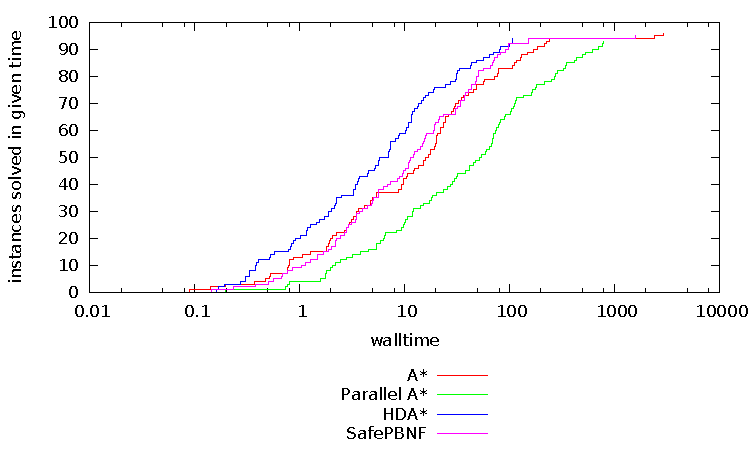
\includegraphics[width=\columnwidth]{competition/15puzzle_vector_walltime.pdf}
		\caption{15 Puzzle (nested bucket)}
		\label{fig:15puzzle_vector}
	\end{subfigure}
	\begin{subfigure}{0.4\columnwidth}
		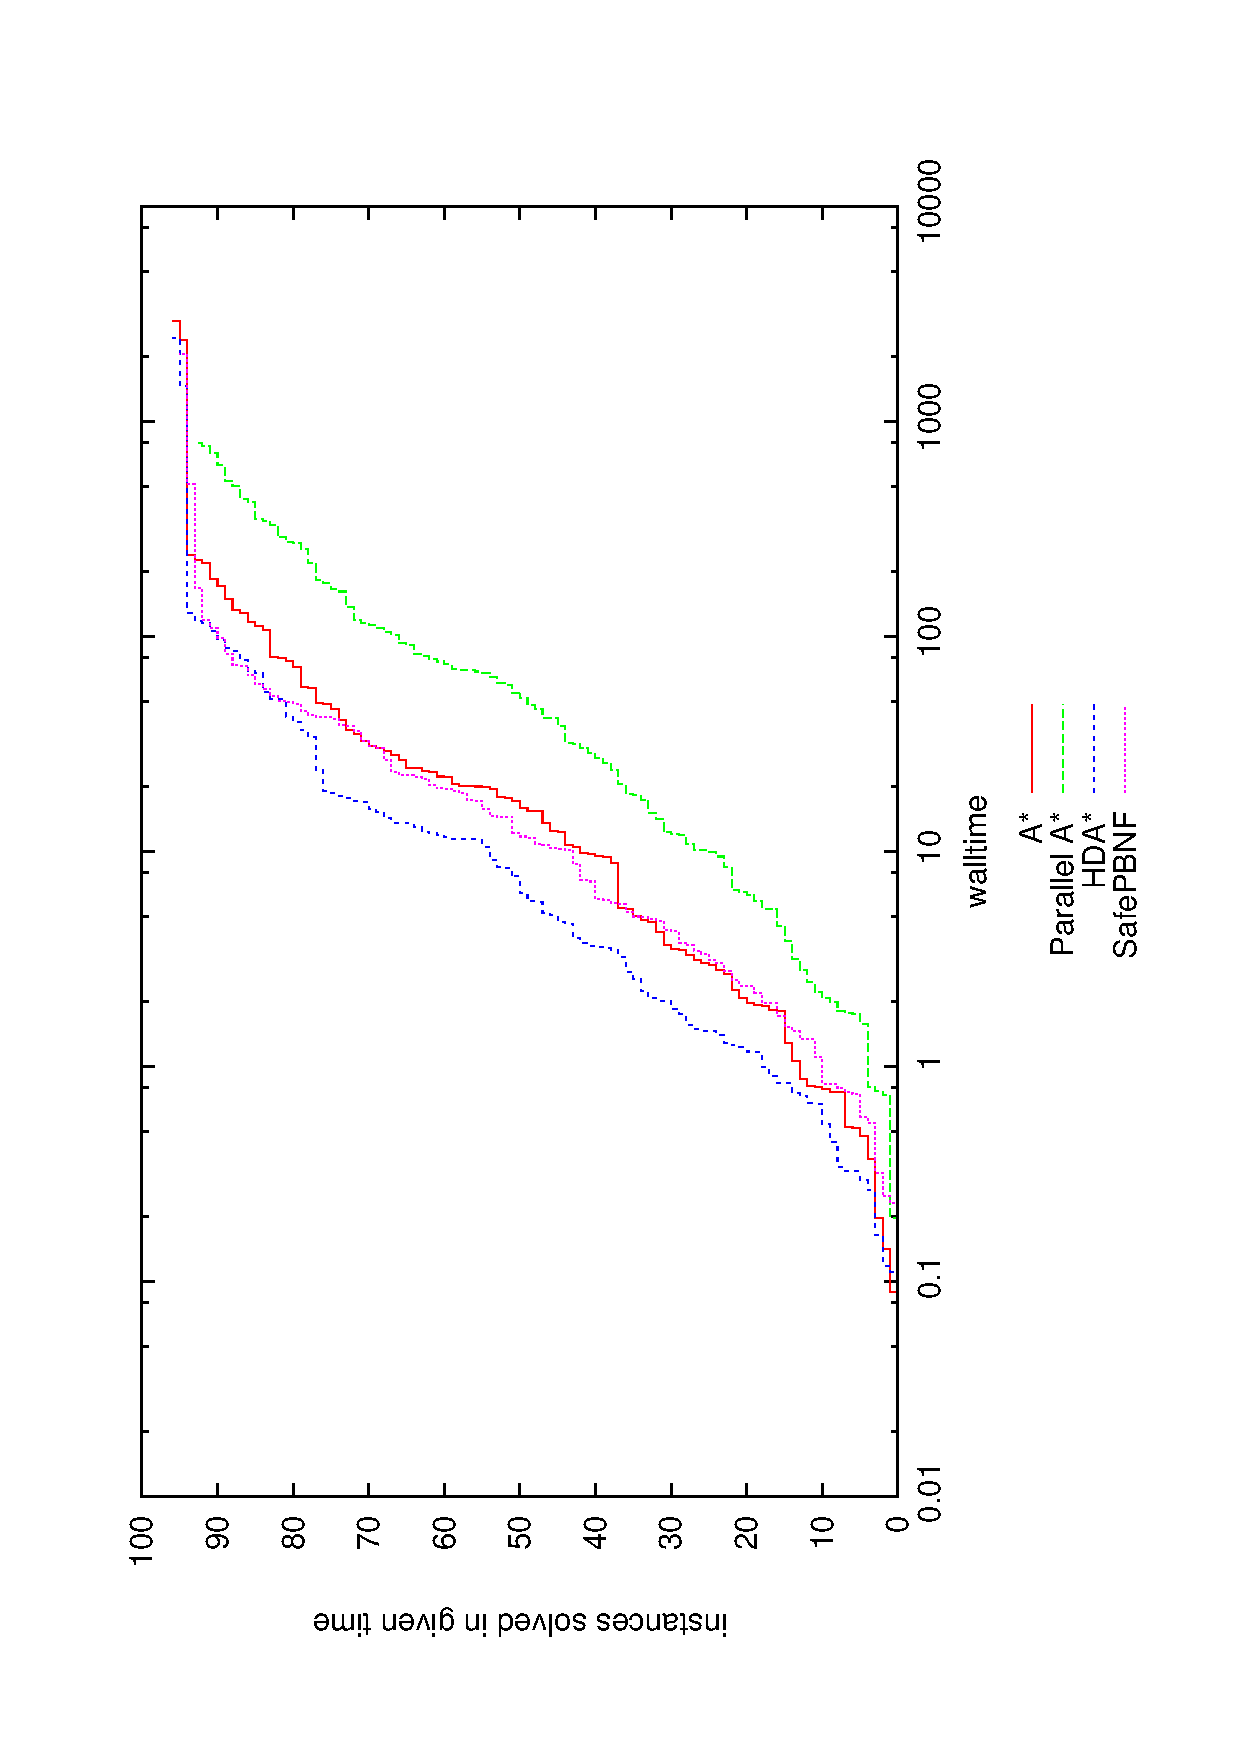
\includegraphics[width=\columnwidth]{competition/15puzzle_heap_walltime.pdf}
		\caption{15 Puzzle (heap)}
		\label{fig:15puzzle_heap}
	\end{subfigure}
	\begin{subfigure}{0.4\columnwidth}
		\includegraphics[width=\columnwidth]{competition/24_walltime.pdf}
		\caption{24 Puzzle (nested bucket)}
		\label{fig:24puzzle_vector}
	\end{subfigure}
	\begin{subfigure}{0.4\columnwidth}
		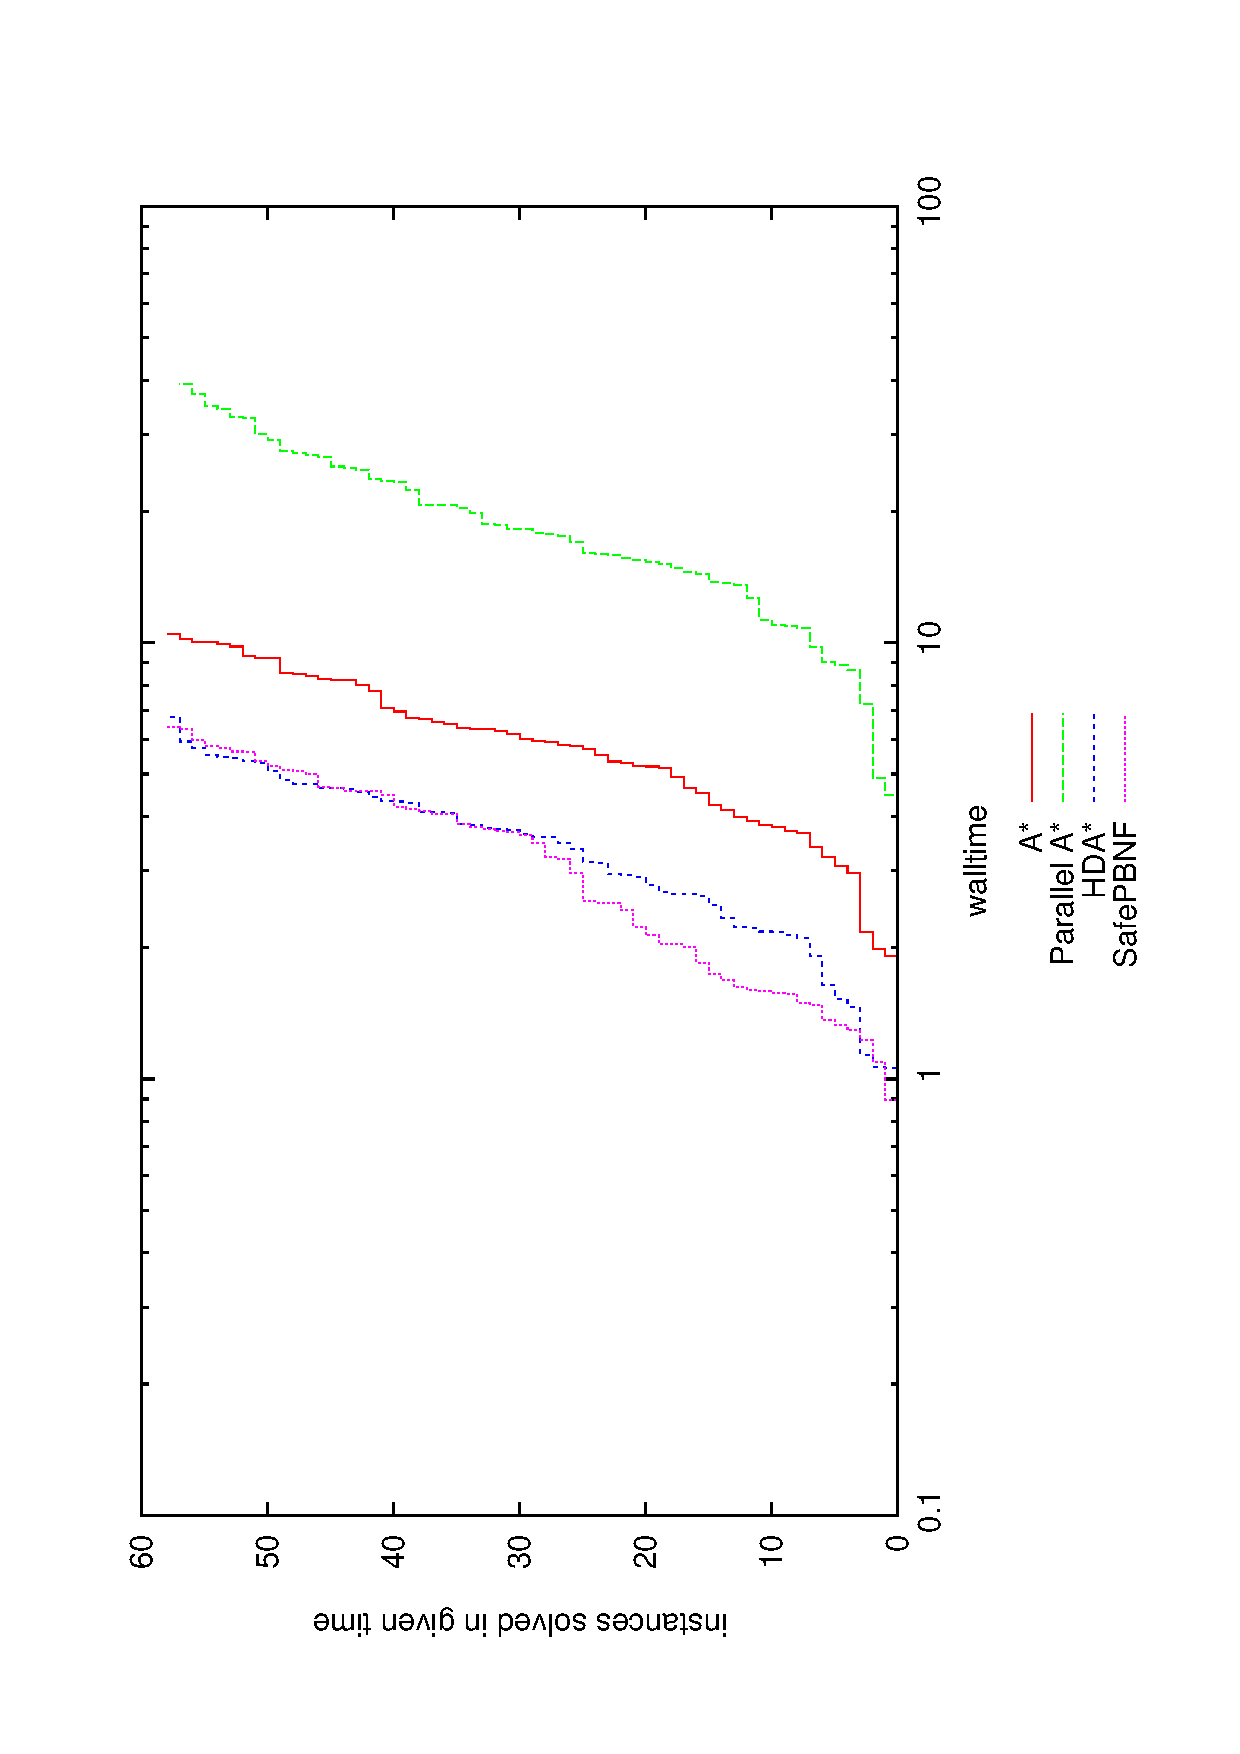
\includegraphics[width=\columnwidth]{competition/grid_walltime.pdf}
		\caption{Grid Pathfinding (nested bucket)}
		\label{fig:grid}
	\end{subfigure}
%	\begin{subfigure}{0.4\columnwidth}
%		\includegraphics[width=\columnwidth]{competition/tsp_20_walltime.pdf}
%		\caption{TSP20 minimum spanning tree (heap)}
%		\label{fig:tsp_20_mst}
%	\end{subfigure}
	\begin{subfigure}{0.4\columnwidth}
		\includegraphics[width=\columnwidth]{competition/tsp_13_walltime.pdf}
		\caption{TSP (heap)} % 13 round trip distance
		\label{fig:tsp_13}
	\end{subfigure}
	\caption{HDA*とSafePBNFの実行時間の比較}
	\label{fig:comparison}
\end{figure}

\begin{figure}[h]
	\centering
	\begin{subfigure}{0.4\columnwidth}
		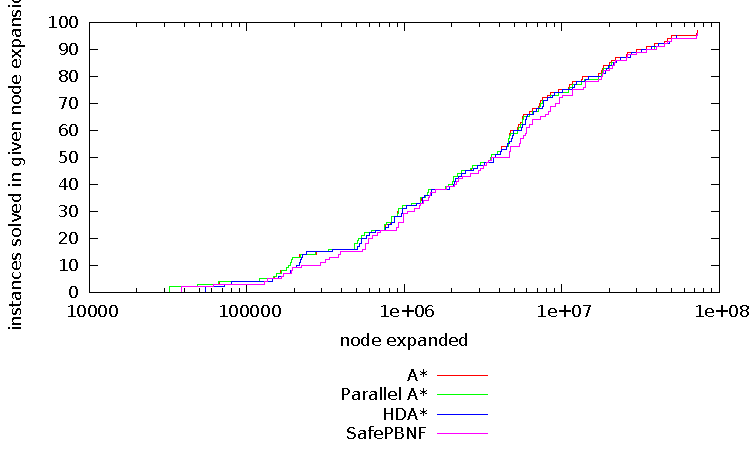
\includegraphics[width=\columnwidth]{competition/15puzzle_vector_expd.pdf}
		\caption{15 Puzzle (nested bucket)}
		\label{fig:15puzzle_vector_expd}
	\end{subfigure}
	\begin{subfigure}{0.4\columnwidth}
		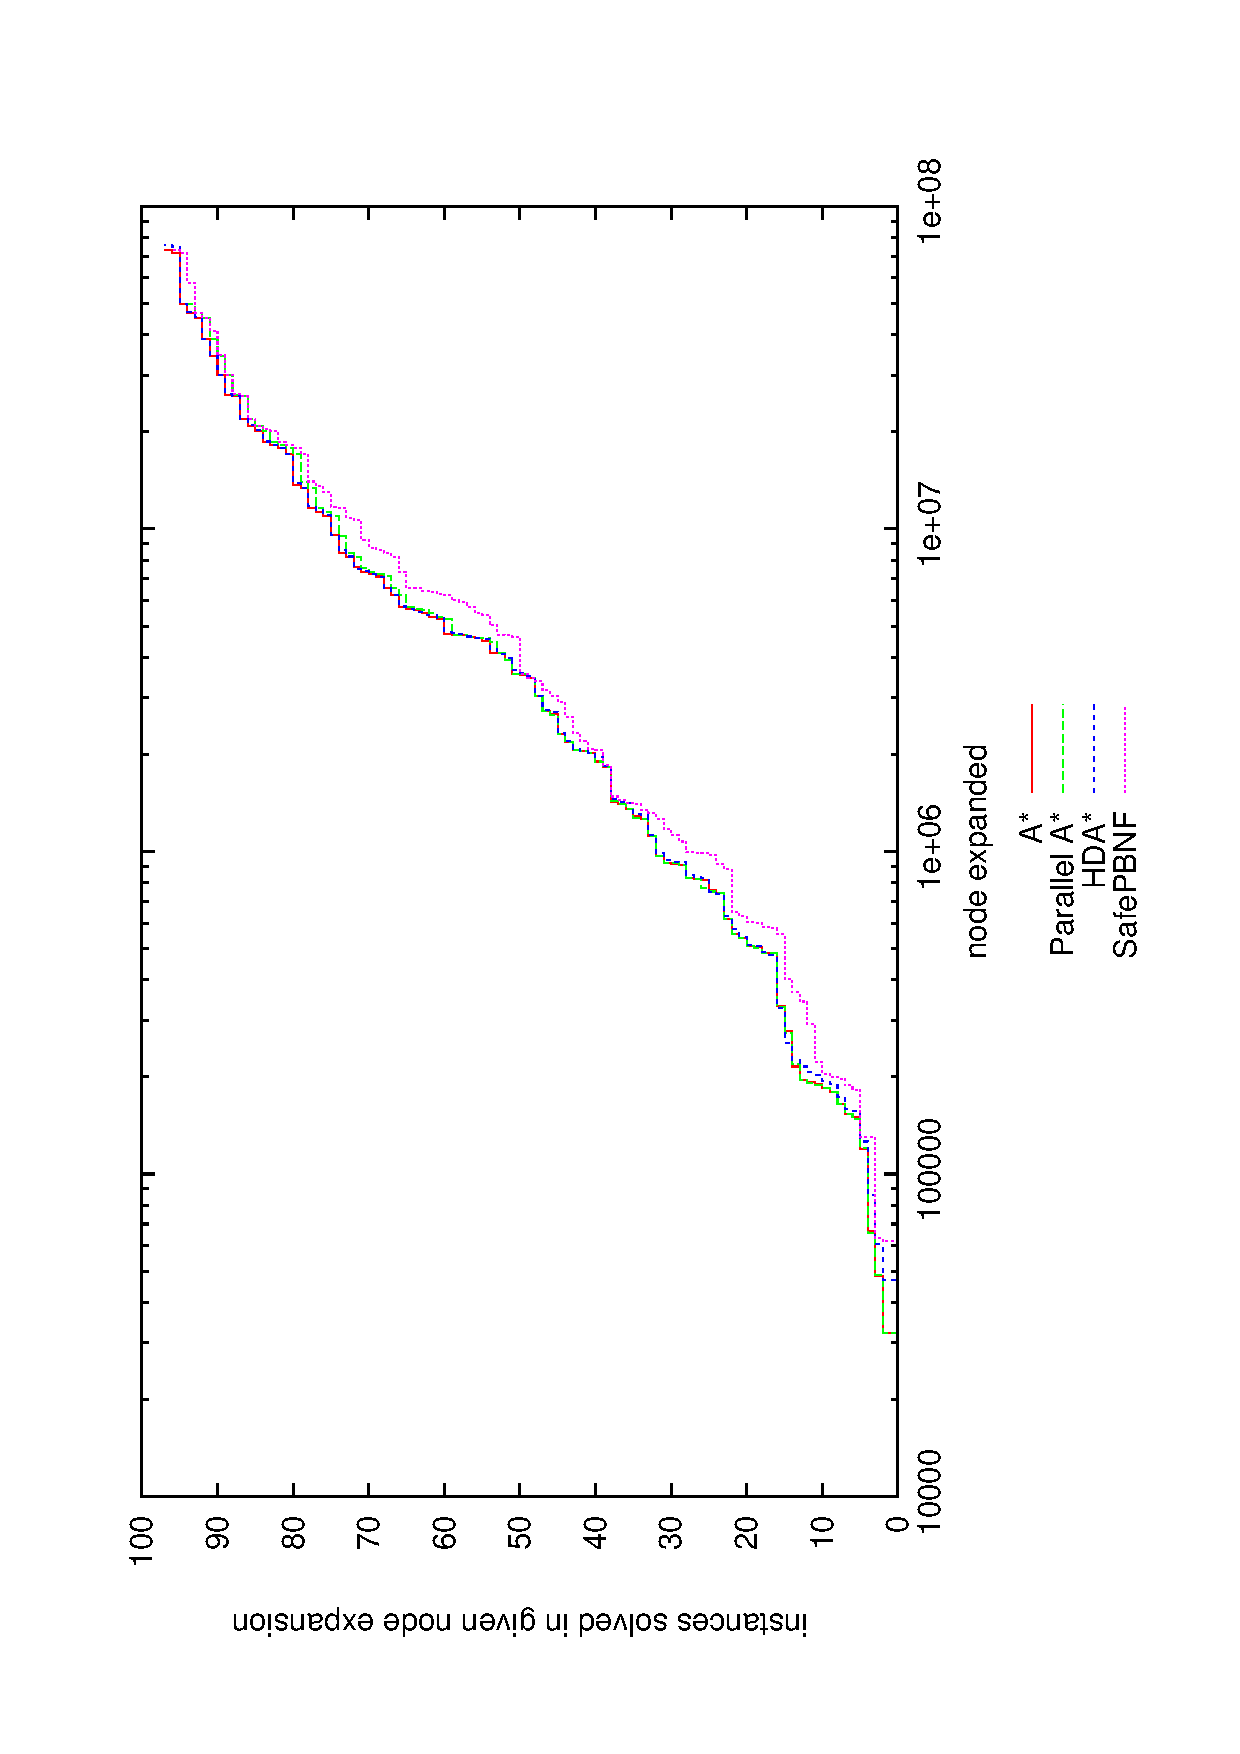
\includegraphics[width=\columnwidth]{competition/15puzzle_heap_expd.pdf}
		\caption{15 Puzzle (heap)}
		\label{fig:15puzzle_heap_expd}
	\end{subfigure}
	\begin{subfigure}{0.4\columnwidth}
		\includegraphics[width=\columnwidth]{competition/24_expd.pdf}
		\caption{24 Puzzle (nested bucket)}
		\label{fig:24puzzle_vector_expd}
	\end{subfigure}
	\begin{subfigure}{0.4\columnwidth}
		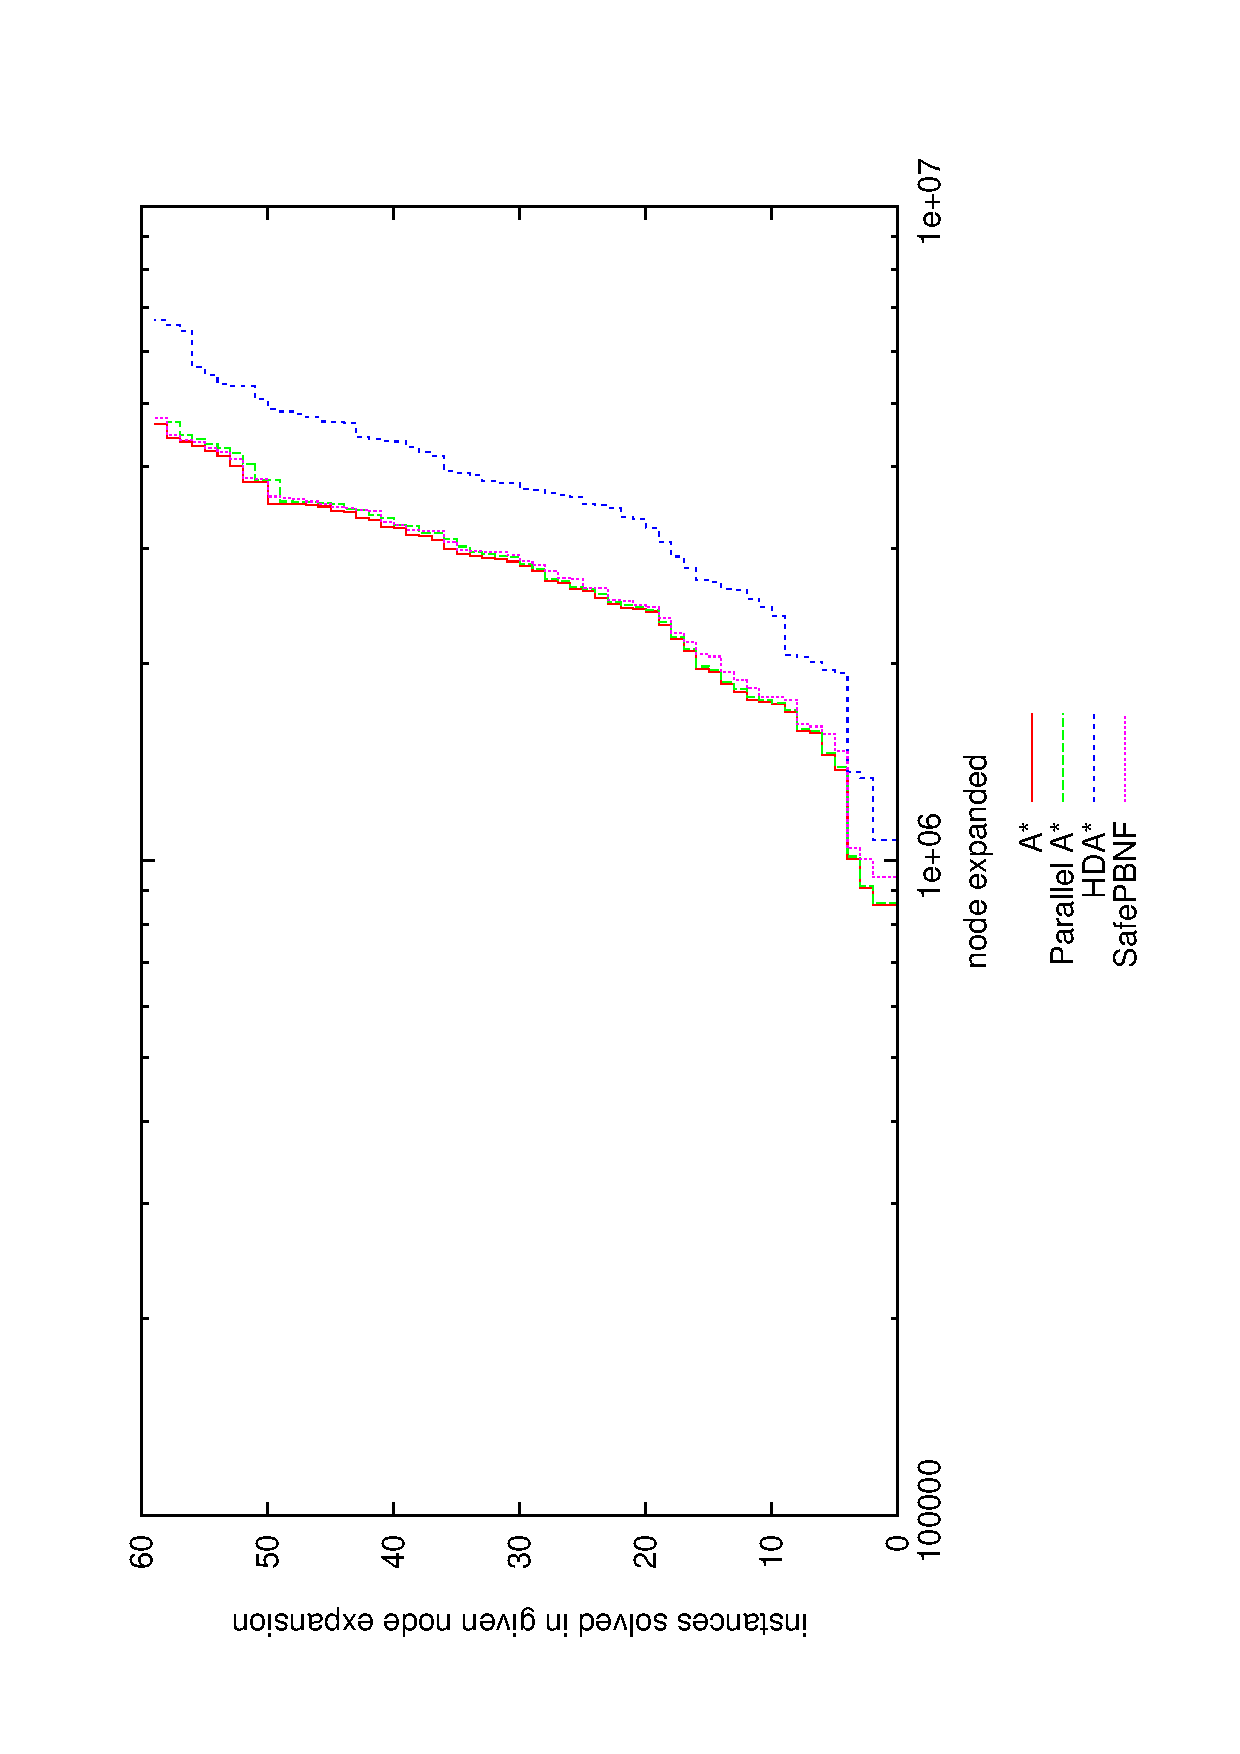
\includegraphics[width=\columnwidth]{competition/grid_expd.pdf}
		\caption{Grid Pathfinding (nested bucket)}
		\label{fig:grid_expd}
	\end{subfigure}
%	\begin{subfigure}{0.4\columnwidth}
%		\includegraphics[width=\columnwidth]{competition/tsp_20_expd.pdf}
%		\caption{TSP20 minimum spanning tree (heap)}
%		\label{fig:tsp_20_mst_expd}
%	\end{subfigure}
	\begin{subfigure}{0.4\columnwidth}
		\includegraphics[width=\columnwidth]{competition/tsp_13_expd.pdf}
		\caption{TSP (heap)} % 13 round trip distance
		\label{fig:tsp_13_expd}
	\end{subfigure}
	\caption{HDA*とSafePBNFの展開ノード数の比較}
	\label{fig:comparison_expd}
\end{figure}%


図\ref{fig:comparison}が実行時間の比較である。それぞれの図は、横軸に実行時間、縦軸にその実行時間内に解ける問題の数を示してある。これらの結果から、特に実行時間の大きい問題ドメイン・インスタンスにおいて、HDA*はSafePBNFよりもパフォーマンスに優れると結論出来る。一方、実行時間が5秒未満程度の小さい問題に対してはSafePBNFの方が優れる場合が多い。\ref{sec:analysis1}章で述べたように、HDA*は実行時間の冒頭と末尾に探索オーバーヘッドがある。実行時間が短い場合、これらのオーバーヘッドの割合が大きくなる。よって、小さな問題インスタンスに対しては探索オーバーヘッドが大きく、SafePBNFの方が速いと考えられる。特にGrid Pathfindingの1秒程度の問題においてHDA*は大きな探索オーバーヘッドを持つ。

図\ref{fig:comparison_expd}は展開ノード数の比較である。それぞれの図は、横軸に展開ノード数、縦軸にその展開ノード数以内に解ける問題の数を示してある。実行時間の短いGrid Pathfindingを除き、HDA* vs. SafePBNFの展開ノード数はあまり変わらない。\ref{sec:analysis1}章の結論とこの結果を踏まえると、HDA*は十分に大きな問題に対しては探索オーバーヘッドの殆どない手法であると結論出来るだろう。BurnsらがHDA*の探索オーバーヘッドを指摘したのはHash関数をSimple Hashで実装したからである。図\ref{fig:order_naive_hash}及び図\ref{fig:hdastar_tuning}より、Simple Hashは明らかに不均一なHash関数である。

図\ref{fig:15puzzle_heap}は15 Puzzleドメインでオープンリストをnested bucketで実装した場合の実行時間の比較である。このドメインはノードの展開が非常に高速なドメインである。この場合でもHDA*は逐次A*に対して高速化が可能である。これは\ref{sec:analysis1}章の実験結果と一致する。一方、SafePBNFは逐次A*に対して高速化が見られない。図\ref{fig:15puzzle_heap}は15 Puzzleドメインでオープンリストをheapで実装した場合の実行時間の比較である。この実験結果はheap実装においてもHDA*がSafePBNFよりもパフォーマンスに優れるということを示す。

nested bucket実装でSafePBNFが速くならない原因は二つの理由が考えられる。一つは、nested bucket実装によってノードの展開が高速化したことである。ノードの展開が高速であると、並列化のオーバーヘッドによる影響が比較して大きくなる。よって、heap実装時には見られなかったオーバーヘッドの影響を受けていると考えられる。もう一つに、そもそもSafePBNFの高速化は主にheapを分割することによるものであった可能性がある。SafePBNFは15 Puzzleの場合3360個のnblockに分割する。よって、オープンリストは1/3360の大きさであると期待される。この時のheapへのアクセス速度の違いは非常に大きいと考えられる。BurnsらはSafePBNF (3360 nblocks)とHDA* (8 threads)のheapへのアクセスにかかるCPU時間の計測を行い、SafePBNFのそれがほぼ0秒であるのに対してHDA*はおおよそ$0.00001$秒(中央値)かかることを示している\cite{Burns2010}。これは1回のアクセスにかかる時間なので、実行時間を通しての合計は非常に大きい。

HDA*でも各スレッドのheapを分割することは可能である。Hash関数による仕事の分配を各スレッド内のheapに自然に流用することが出来る。よって、HDA*でも分割heapを用いることで実数コストドメインにおけるパフォーマンスを向上させることが出来ると考えられる。これは今後の研究課題である。

% PBNFが速いのは単にheapを分割しているからだけでは?

%Minimum Spanning Treeは計算時間の大きいヒューリスティックである。その為TSP20はノードの展開が遅い。この時、

\begin{table}[h]
	\centering
	\begin{tabular}{lrrrr} \hline
		 & &             HDA* & & SafePBNF \\ 
		 &  解の発見回数 & 最初の解の発見時間 & 解の発見回数 & 最初の解の発見時間 \\ \hline
		15 Puzzle (nested bucket)& 1 & 14.56 & 1.14 & 20.73 \\ 
		24 Puzzle & 1 & 59.82 & 1 & 67.04 \\ 
		Grid Pathfinding & 1.02 & 3.45 & 1.02 & 3.30 \\ 
%		TSP20 MST & 1 & 5.18 & \textbf{2.25} & \textbf{1.23} \\ 
		TSP13 RTD & 1 & 16.80 & \textbf{2.60} & \textbf{8.56} \\ \hline
	\end{tabular}
	\caption{解の発見回数と最初の解の発見時間の平均}
	\label{hdastar_incumbent}
\end{table}

% TSPはSafePBNFが得意な問題ドメインであると考えられる。空間を簡単に分割することが出来る為である。

SafePBNFはTSPドメインにおいて効率的である。その理由としては以下の二点が考えられる。一つは前述のheapを分割することによる高速化である。もう一つはドメインに解が無数にあるからである。表\ref{hdastar_incumbent}はHDA*とSafePBNFにおいて、解を発見した平均の回数である。SafePBNFの探索方法はAnytime Searchのような特徴を持つ\cite{Burns2010}。すなわち、SafePBNFは最適でない解を素早く見つけ、時間と共により良い解を発見することが出来る。最適でない解を発見した場合、その解のコストよりもコストの大きいノードを生成する必要がなくなる。ノードの生成は探索時間の大きな割合を占める為、生成の回数を減らすことは大きな高速化につながる。TSPは深さが都市の数と同じノードは全て解である。都市が13個の場合は$12!$通りの解が存在する。SafePBNFは解が無数にあるTSPでは素早く解を発見でき、その為最適解も高速に見つけられると考えられる。

どのドメインにおいてもシンプルなParallel A*は逐次A*よりも遅くなってしまう。Parallel A*はオープンリストとクローズドリストにロックを必要とする。スレッドはロックが解放されるのを待たなければならない為、大きな同期オーバーヘッドが生じる。この結果はBurnsらの実験と一致する\cite{Burns2010}。なお、Parallel A*は24 Puzzleを解けなかった為実行結果を省略してある。
\newline

\section{おわりに}
\label{sec:conclusion}

本研究の貢献は大きく分けて2つある。

\begin{enumerate}
\item HDA*の探索オーバーヘッドの定性的な分析
\vspace{3mm}

HDA*の探索オーバーヘッドの原因を三つに分類を行い、十分問題サイズが大きい場合に探索オーバーヘッドが無視出来る程度に小さいことを理論的に示した。また、高速化効率と探索オーバーヘッドを問題インスタンス毎に示すことで、それを実験的にも証明した。本研究は共有メモリ環境において行われたが、分散メモリ環境においても同様の結果が得られると推測している。その実験的な実証は今後の研究課題である。また、本研究は新しい探索オーバーヘッドの分析手法を示した。これは他の並列探索においても有効な分析方法であると考えられる。
\newline

\item HDA*とPBNFの再評価
\vspace{3mm}

先行研究の分析の問題点を指摘し、より詳細でミクロな分析を行った。実験により、マルチコア環境においても相応しい実装を行えばHDA*の方がパフォーマンスに優れるという結果を得た。また、本研究ではOptimal Searchを対象としたがSuboptimal Searchにおける実験は行っていない。Suboptimal Searchにおける性能比較は今後研究課題である。簡易ヒューリスティックを用いたTravelling Salesperson ProblemにおいてはSafePBNFの方がHDA*よりも速いという結果を得た。これはSafePBNFのheapの方が小さい為、heapへのアクセスが速い為ではないかと考えられる。


\end{enumerate}

\newpage
\section{謝辞}

研究室の先輩方にはミーティングや中間発表などで沢山の有益なアドバイスを頂きました。特に同期の堀江君とは本当に毎日議論を重ね、沢山のことを学ばせて頂きました。指導教員である福永先生には、初めて情報科学に触る私に対してとても丁寧にご指導して頂きました。研究とは、情報科学とは、プログラミングとは、あらゆることを教えて頂きました。何よりも、研究が楽しいということを教えて頂いたことに深く感謝致します。修士課程でも、一つでも多くのことを学ばせて頂きたいと思います。

\newpage

\bibliographystyle{junsrt}
\bibliography{b}

\newpage

\printindex

\end{document}
